\documentclass[english,11pt]{article}

\usepackage[T1]{fontenc}
\usepackage[utf8]{inputenc}
\usepackage{hyperref}
\usepackage{graphicx}
\usepackage{babel}
\usepackage{color}
\usepackage{caption}
\usepackage{subcaption}
\usepackage{float}
\usepackage{titlesec}
\usepackage{fancyhdr}
\usepackage{enumitem}
\usepackage{fix-cm}
\usepackage{amssymb}
\usepackage{adjustbox}
\usepackage{longtable}
\usepackage{amsmath}

\graphicspath{{./images/}}

\title{\textbf{Introduction to Neuroinformatics}
				\\Summary of the lectures 2013\\\normalsize Version 2.0}

\author{
\texttt{Initial Version 2012}\\
  Benjamin Ellenberger
  \and
   \texttt{Revision 2013}\\
  Joachim Ott\\Dora Sumisławska}

\date{}
\newcommand{\sectionbreak}{\clearpage}
\begin{document}

\maketitle
\thispagestyle{empty}

\clearpage
\pagenumbering{roman}
\tableofcontents



\clearpage
\pagenumbering{arabic}


\pagestyle{fancy}
\fancyhead[R]{} % predefined ()

\fancyhead[L]{\fontsize{10}{12}\selectfont \leftmark} % 1. sectionname
\rfoot{\thepage}
\cfoot{} % get rid of the page number 
%\renewcommand{\headrulewidth}{0pt}
\renewcommand{\footrulewidth}{0pt}
% The paper headers







\section{Lecture 1 - Neuroinformatics (Michael Pfeiffer)}
% Version Dora:

\subsection{Introduction}
\begin{itemize}

\item Why do we have the brain?

\begin{figure}[htbp]
\centering
  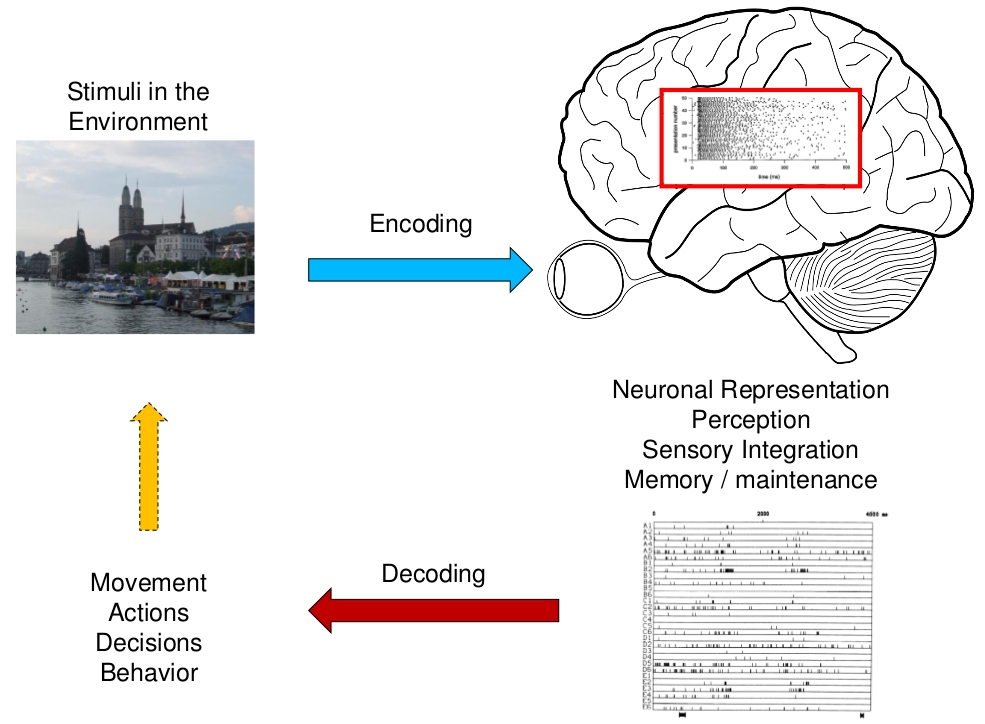
\includegraphics[scale=0.45]{images/1_1.jpg}
  \label{fig:1_1}
\end{figure} 

\item Alan Turing \\
John von Neumann

\begin{figure}[htbp]
\centering
  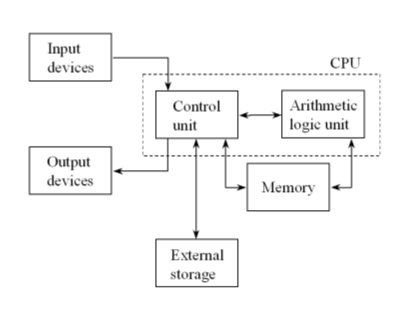
\includegraphics[scale=0.6]{images/1_2.jpg}
  \label{fig:1_2}
\end{figure} 

\newpage
\item How is a brain different/ similar to a computer?

Similar: \\ Process information, Logical operations, Memory, Use electrical (digital) signaling, Can learn from inputs, Consume energy,
 ...

Different:\\ Massive parallelism, Constantly adapting, Chemical signaling, Unreliable units, Analog computation, Robust to damage, Very energy efficient, ...

\begin{figure}[htbp]
\centering
  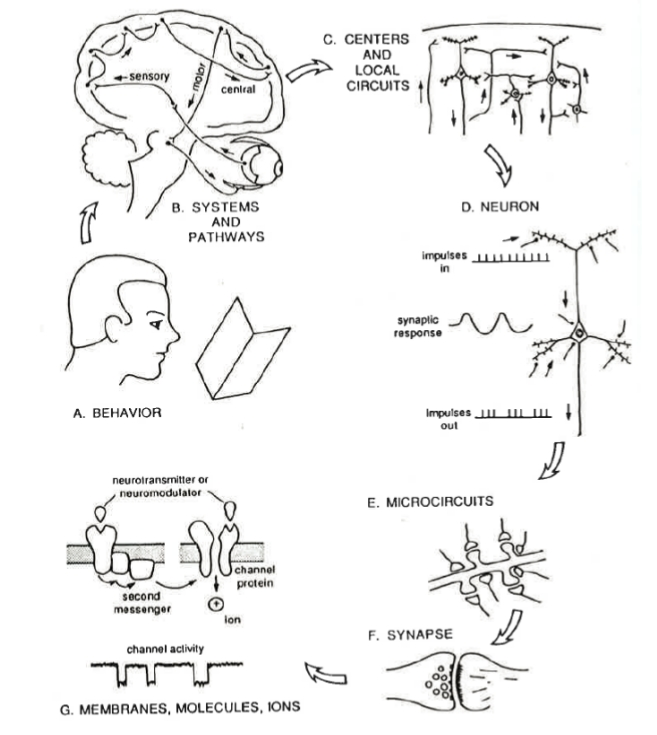
\includegraphics[scale=0.7]{images/1_3.jpg}
  \label{fig:1_3}
\end{figure} 

\newpage
\item What this course will be about?

Information processing in the brain: neurons,
synapses, nervous system organization;
Analytical descriptions of neural computations;
Learning and plasticity;
Encoding information in the brain;
Theoretical neural network models;
Engineering brain-like computers.

MIPS = million instructions per second

Tianhe world's fastest computer, match only 1\% of your brain ($\approx 85$ Billion Nerve Cells)

Windows XP $\approx 1.5 GB $ of code, human genome ($\approx 750 MB$).

\item The era of "Big Brain Projects" in ex. Human Brain Project. 

Neurogrid -- real-time emulation on 1 Mio. neurons

\end{itemize}





\newpage
\section{Lecture 2 - Nervous System Organization (Kevan Martin)}


% Version Benjamin reviewed by Dora:
\subsection{Building elements of the brain}
Brain consists of:
\begin{itemize}
\item Forebrain (Prosencephalon)
\subitem Cortex
\subitem Thalamus ('couch')
\subitem Hippocampus
\subitem Basal Ganglia
\subitem Corpus Callosum
\item Midbrain (Mesencephalon)
\subitem Tectum
\subitem Tegmentum
\item Hindbrain (Rhombencephalon)
\subitem Cerebellum (Computantionally mysterious)
\subitem Pons
\subitem Medulla Oblongata

\item Whitematter
\subitem Glia cells, myelinated axons
\item Greymatter
\subitem Neurons (Soma)
\end{itemize}

\begin{figure}[H]
        \centering
        \begin{subfigure}[b]{0.5\textwidth}
                \centering
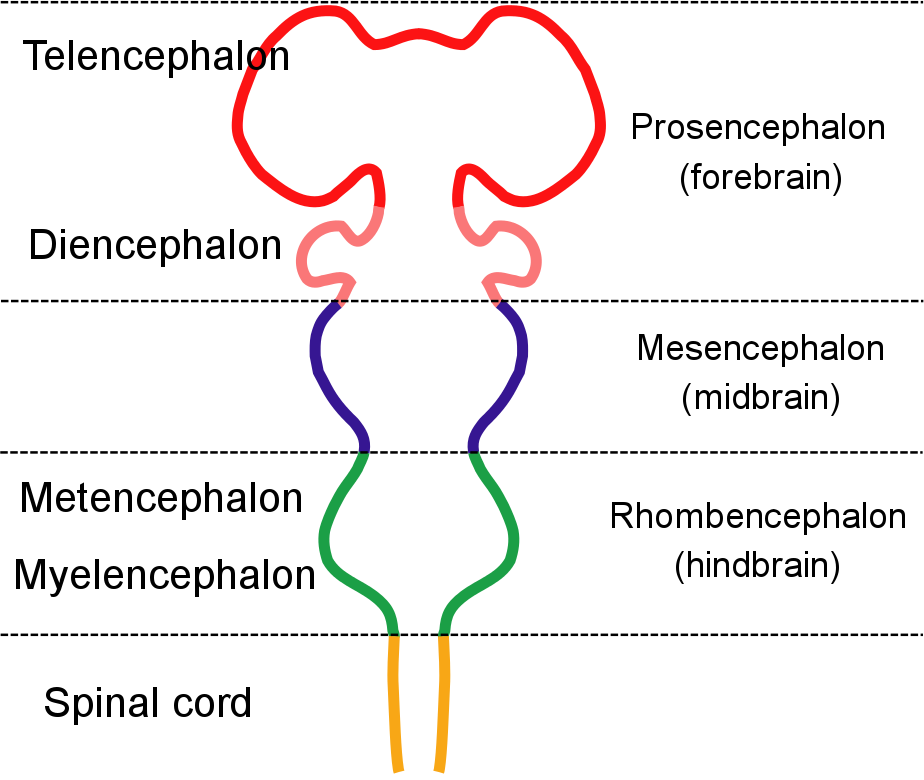
\includegraphics[width=\textwidth]{brain-parts.png}
        \end{subfigure}%
        ~
        \begin{subfigure}[b]{0.5\textwidth}
                \centering
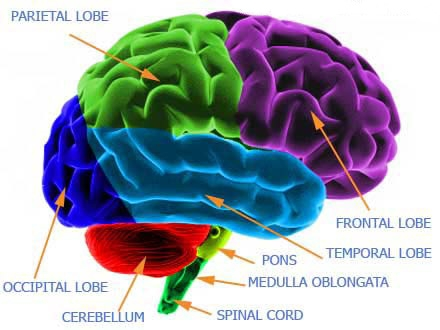
\includegraphics[width=\textwidth]{brain.png}
        \end{subfigure}
\end{figure}
\begin{figure}[H]
        \centering
        \begin{subfigure}[b]{0.5\textwidth}
                \centering
				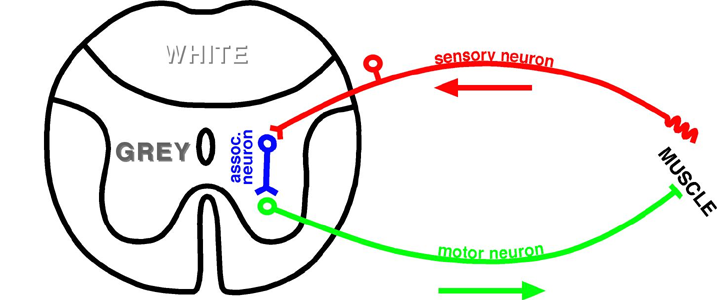
\includegraphics[width=\textwidth]{motor-sensory-neuron.png}
        \end{subfigure}%
        ~
        \begin{subfigure}[b]{0.5\textwidth}
                \centering
				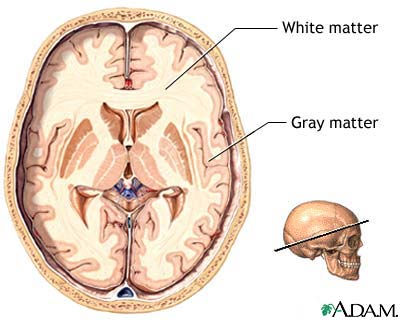
\includegraphics[width=\textwidth]{brain-cut.png}
        \end{subfigure}
\end{figure}

\subsection{Nervous System in numbers}
White matter $1mm^3\rightarrow$ 9m of wires (axons).\\
Grey matter $1mm^3\rightarrow$ 50'000 neurons, 4km of wires. 
$\rightarrow$ Long distance communication needs space.\\
Only 1m goes to spinal cord.\\
100k cells in $1 mm^3$.\\
Auditory vs visual pathway from sensor 1.2 m to 15km.






\newpage
\section{Lecture 3 - Membrane Potential (Kevan Martin)}


% Version Benjamin (Douglas) reviewed by Dora:
\subsection{Membrane Potential - Structure and Function}
The membrane bilayer creating the energy barrier (ion can not just flow through it without channels or pumps) between: 
\begin{itemize}
\item ECS (Extra cellular solution)
\item ICS (Intra cellular solution)
\end{itemize}

is built out of two types of molecules:
\begin{itemize}
\item the charged hydrophilic dipole head-group (hydrophile -- funs of water -- water molecules are also polarised),
\item uncharged, hydrophobic (with phobie of water) hydrocarbon tails turning inward, avoiding contact with water.
\end{itemize}

\begin{figure}[h]
\begin{center}
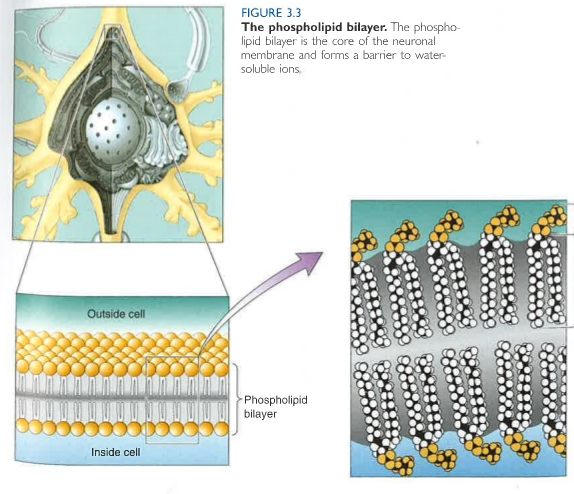
\includegraphics[scale=0.8]{images/3_1.jpg}
\end{center}
\end{figure}


Transmembranal proteines play an important role as they have charged ends(phosphate heads) and uncharged bodies and therefore fit inside of the membrane as it aligns with the uncharged inner part of the membrane and with the outer charged parts.


\begin{figure}[h]
\begin{center}
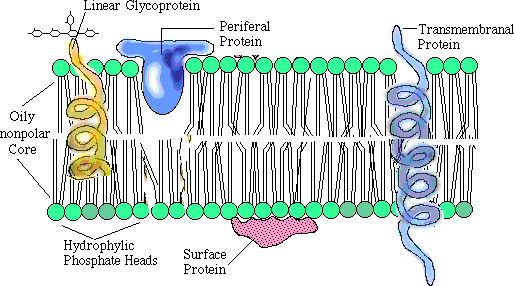
\includegraphics[width=0.9\textwidth]{bilayer-closeup.png}
\end{center}
\end{figure}

The spike is the action potential caused by sodium ($Na^{2+}$) and changes in the membrane conductance. This shows that there is a voltage source in the membrane.

\begin{figure}[h]
\begin{center}$
\begin{array}{cc}
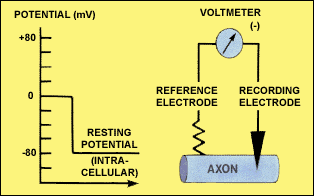
\includegraphics[width=0.5\textwidth]{voltage-source-in-membrane.png}

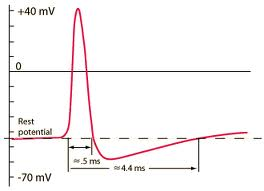
\includegraphics[width=0.5\textwidth]{voltage-source-in-membrane2.png}

\end{array}$
\end{center}
\end{figure}

There are 2 basic mechanisms for the membrane potential leading to equlibrium (resting potential):
\begin{itemize}
\item Active mechanisms ($Na^+$/$K^+$-Pump from ECF to ICF).
\item Electrical force -- in order to keep the difference in ion concentrations in ECF, ICF (asymmetry across membrane) there is a negative potential with reference to extracellular potential. Because in the rest there is only potassium ion flows we concentrate on them. Negative potential in ICF attracts positive charged $K^+$ ions into the cell while due to diffusion they are likely to leave the cell -- inside grater concentration.
In this way both forces are balanced.
\end{itemize}

\subsection{Concentrations across the membrane}

\begin{center}
\begin{tabular}{ l | c | r }
 ION	& ICF & ECF \\
  $Na^+$(Sodium) & - & + \\
  $K^+$(Potassium) & + & - \\
  $Cl^-$(Chlorine) & - & + \\
  $Ca^{2+}$(Calcium) & x & (+) \\
  Large Anions(not passing membrane) & + & (-) \\
\end{tabular}
\end{center}

There is a concentration gradient top-down from high concentration to low concentration. The pump uses ATP to build up the gradient if it is released.

There are different structures enabling proteins to cross the membrane. 
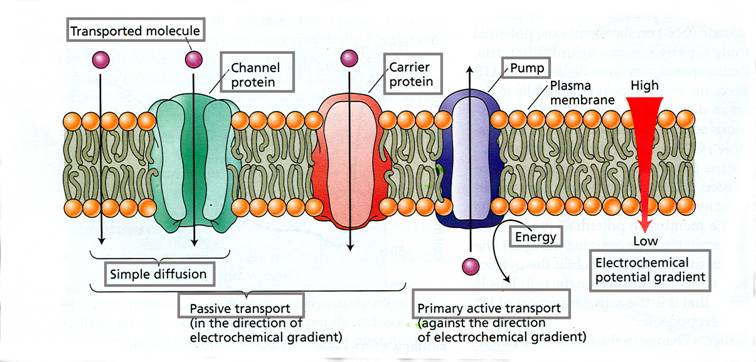
\includegraphics[width=\textwidth]{bilayer-closeup2.png}


\subsection{Nernst equation}

\begin{equation}
E_{ion}= \frac{RT}{zF} \cdot ln (\frac{[Ion]_{extracellular}}{[Ion]_{intracellular}}) 
\end{equation}




\begin{itemize}
\item R Universal gas constant ($8.3144 \frac{J}{mol \cdot K}$)
\item F Faraday constant ($ 96500 \frac{C}{mol}$)
\item z number of electrons involved in the reaction
\item one mole = 6.02e23, solution is one molar when its concentration is $1 \frac{mole}{liter}$
\end{itemize}

$At 37^\circ C :$

\begin{equation}
E_{ion} \approx 60 mV \cdot ln ({\frac{[Ion]_{extracellular}}{[Ion]_{intracellular}}}) 
\end{equation}



\subsection{Goldman-Hodgkin-Katz equation (GHK-Voltage equation)}

\begin{equation}
\Delta V = \frac{RT}{zF} ln(\frac{P_K[K^+]_{out} + P_{Na}[Na^+]_{out} + P_{Cl}[Cl^{-}]_{in}}{P_K[K^+]_{in} + P_{Na}[Na^+]_{in} + P_{Cl}[Cl^{-}]_{out}})
\end{equation}

This is only for static situations but gives us a sense of how it is actually working.
Basic assumptions:
\begin{itemize}
\item Ion flux obeys Nernst/Planck equation
\item Ions move across membrane independently (no interaction)
\item Electric field in the membrane is constant $E = -\frac{\delta V}{\delta x} = - \frac{\Delta V}{l}$
\end{itemize}







\newpage
\section{Lecture 4 - Passive (Cable) Membrane Properties (Valerio Mante)}


% Version Benjamin (Douglas) reviewed by Dora:
\subsection{Summary of membrane properties:}
\begin{itemize}
\item $J_{diff}$ and $J_{drift}$ are in an equilibrium ($V_m =$ resting potential),
\item Resting potential is due to $K^+$ asymmetric concentration,
\item GHK-equation enables to calculate $\Delta V = $ Difference in Potential across the membrane,
\item if for all ions crossing the membrane $P(Permeability) = 1 \rightarrow Nernst-equation$,
\item 
In great approximation for passive membrane (only potassium and a little bit of sodium channel can cross the membrane) the resting potential is The function of conduction is approximatelly a weighted mean of equlibrium potentials for ions that can cross it. Membrane is not only permeable to potassium ions. There is also steady leak of sodium ions.
\end{itemize}
\begin{equation}
E_m = \frac{g_K E_K+g_{Na} E_{Na}}{g_K+g_{Na}} \approx -65 mV
\end{equation}



\subsection{Electrical nature of the membrane}
 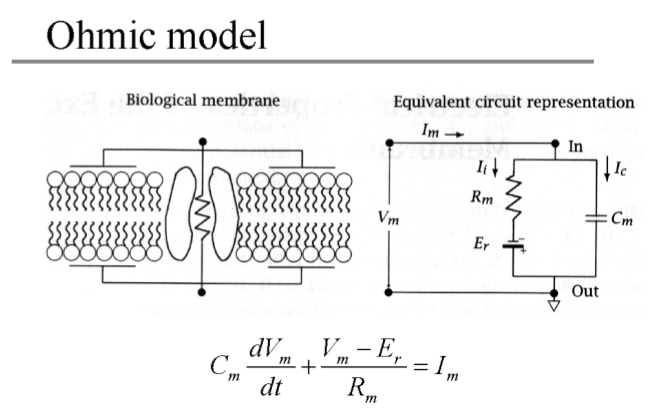
\includegraphics[scale = 0.5]{ohmic-model.png}
 
\begin{itemize}
\item The conductance of the membrane indicates its temporally dynamic character.
\end{itemize}
\begin{equation}
 g_m = \frac{Current}{Voltage} = \frac{1}{Resistance} = \frac{I}{U} = \frac{1}{R_m}
 \end{equation}
 
 \begin{itemize}
\item $I_c + I_o = I_m$
\item If $\frac{\delta V_m}{\delta t} = 0 \rightarrow$ membrane is at rest.
\item Changing the permeability of the membrane results in changable conductance $g(t)$.
\item Temporal summation of the membrane potential.
\end{itemize}

\begin{equation}
V(t) = V(\infty) + (V_{(0)}-V_{(\infty)}) e^{-\frac{t}{RC}}
\end{equation}


%\begin{figure}[H]
%        \centering
%        \begin{subfigure}[b]{0.5\textwidth}
%                \centering
%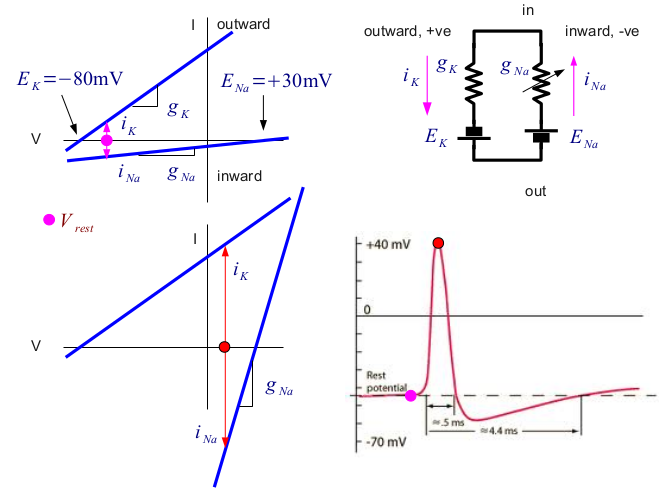
\includegraphics[width=\textwidth]{ohmic-model2.png}
%        \end{subfigure}%
%        ~
%        \begin{subfigure}[b]{0.5\textwidth}
%                \centering
%				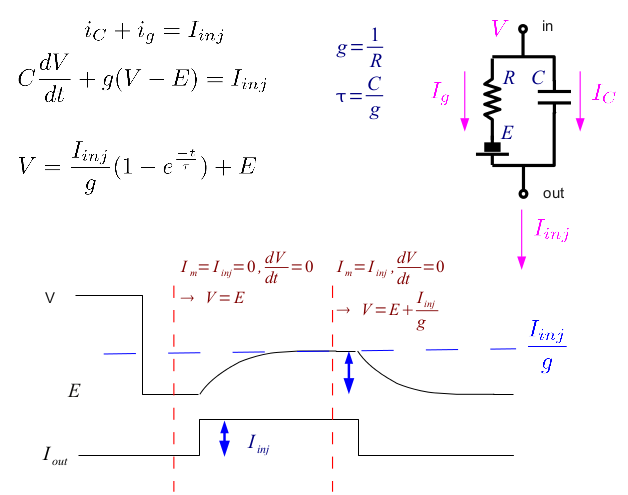
\includegraphics[width=\textwidth]{ohmic-model3.png}
%        \end{subfigure}
%\end{figure}
%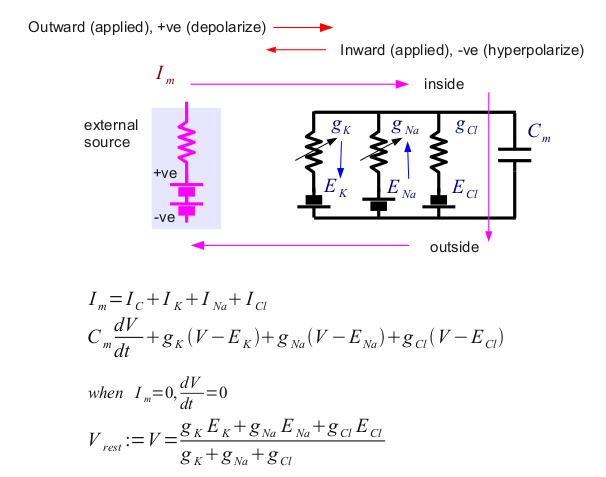
\includegraphics[width=0.5\textwidth]{electrical-membrane.png}
%\begin{itemize}
%\item Typical values for electrical properties of membranes:
%\item Capacitance(Cell of $20\mu m$ diameter: $c_m =C_m \cdot A = 1\frac{\mu F}{cm^2} \cdot 10^{-5} \approx 10 pF$\\
%Resistance:$r_m = \frac{R_m}{A} = \frac{10k\Omega\cdot cm^2}{10^{-5}} \approx 1000 M\Omega$\\
%Time constant($\mu F \cdot M\Omega = sec$): $\tau_m = c_m r_m = \frac{R_m}{A}\cdot C_m A = R_m C_m \approx 10^{-6} \mu F \cdot 10^4\Omega = %10msec$
%\item Membrane behaves like a resistance network\\
%Current leaks out through membrane resistance\\
%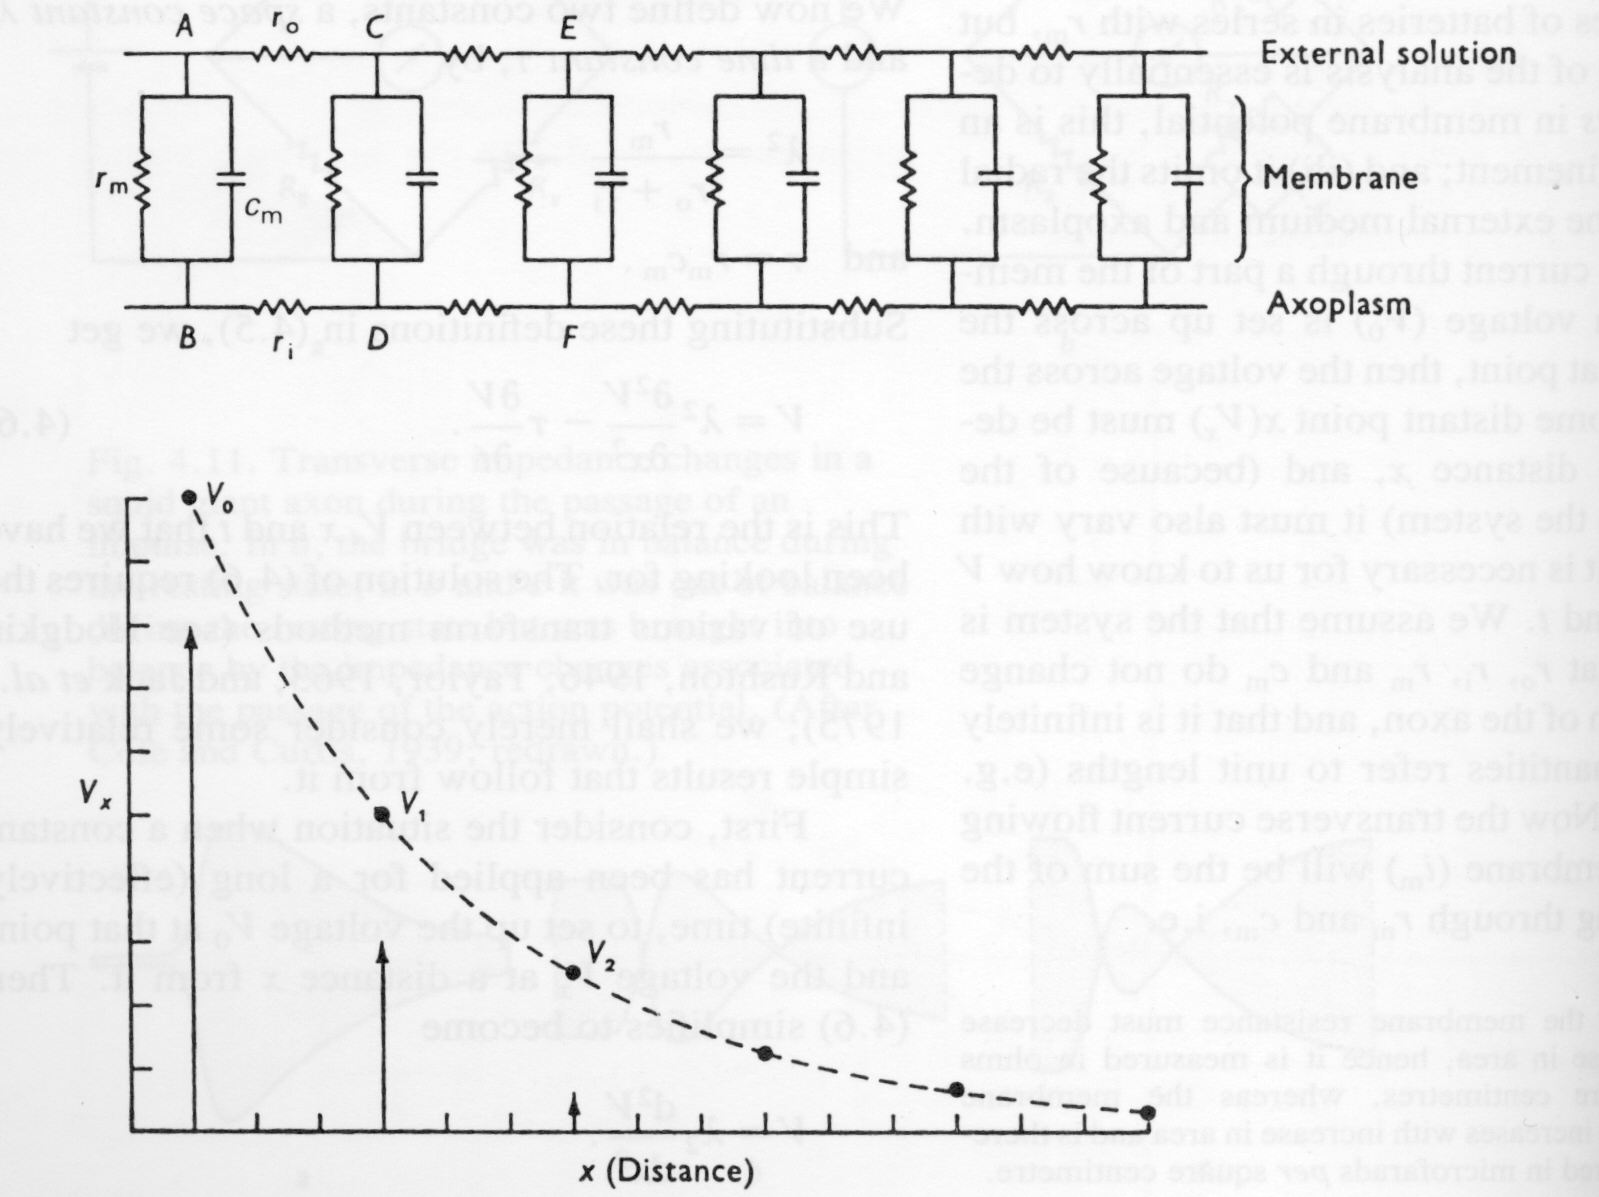
\includegraphics[width=0.6\textwidth]{membrane-leakage.png}\\
%Voltage leakage is rising exponentially. 4 decay constants leads to $\approx 0 V$
%\end{itemize}

\subsection{The cable equation}
For a passive membrane, the membrane potential $V(x, t)$ is determined by solving the following partial differential equation:
\begin{equation}
\tau _m (\frac{\delta v}{\delta t})= \lambda ^2 (\frac{ \delta^2 v}{\delta x^2}) - v + r_m i_e 
\end{equation}

where: 

$\tau_m = (r_m c_m)$ sets the scale for the temporal variation in the membrane 

potential

$a = $ radius of the axon ($= 2 \mu m$)

$v = V - V_{rest}$

$r_m = $ specific membrane resistance $(= 1 M\Omega \cdot mm^2)$

$r_L = $ longitudinal resistnace $(= 1 k\Omega \cdot mm)$

$i_e = $ the current injected into a cell

$\lambda = \sqrt (\frac{a r_m}{2 r_L})$ sets the scale for the spatial variation in the membrane potential ($\lambda$ is called the \textit{electronic length})\\
$\lambda = 0.6mm$ means no signal left after $0.6mm$\\
$\rightarrow$ Increasing $R_m$ of the cable increases $\lambda$\\
$\rightarrow$ Increasing diameter of the cable increases $\lambda$

For the steady-state solution ($\frac{\delta v}{\delta t} = 0$) of the equation then is:

\begin{equation}
v(x) = (\frac{i_e R_\lambda}{2}) e^{-|x|/\lambda},  ~~where R_\lambda = \frac{r_L \lambda}{\pi a^2}
\end{equation}


%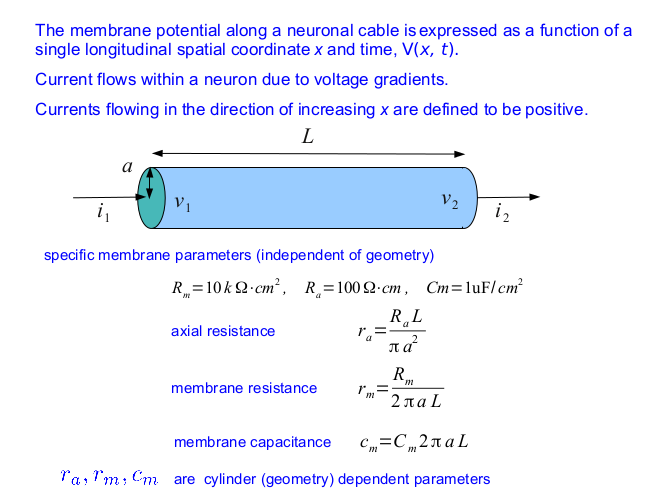
\includegraphics[width=0.9\textwidth]{cable-equation1.png}
%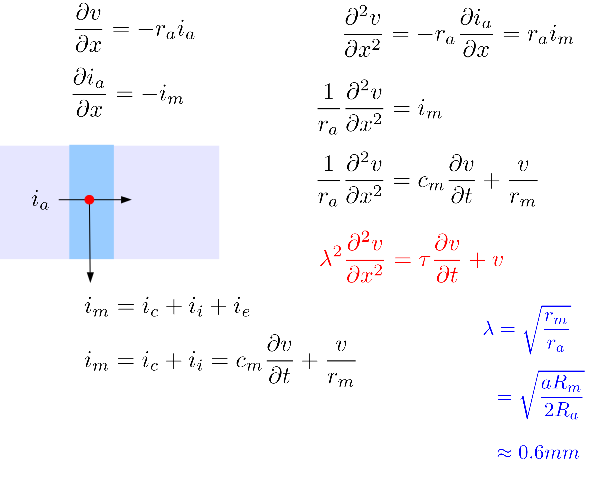
\includegraphics[width=0.9\textwidth]{cable-equation2.png}
%$\tau$ = time constant\\
%$\lambda$ = space constant for $R_m$ and $R_a$ of this cable.\\
%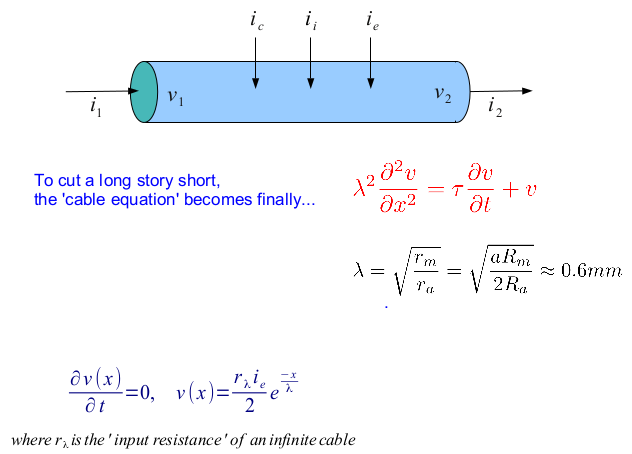
\includegraphics[width=\textwidth]{cable-equation3.png}

%\subsection{From exercises:Electric laws}
%\begin{itemize}
%\item Kirchhoff's Current Law (KCL): The sum of all currents entering and leaving any node in a circuit is not zero.
%\item Kirchhoff's Voltage Law (KVL): The sum of all voltages around a closed loop is zero.
%\item Ohm's Law: $V = I \cdot R$
%\end{itemize}

\subsection{The Hodgkin-Huxley Model}

This is a model that describes how action potentials in neurons are initiated and propagated. is a set of differential equations that approximates the electrical characteristics of excitable cells. The Hodgkin-Huxley model for genration of an action potential:

\begin{equation}
I_{ionic}= g_L (V_m - E_L) + \overline{g_K} \cdot n^4 \cdot (V_m - E_K) + \overline{g_{Na}} \cdot m^3h \cdot (V_m - E_{Na})
\end{equation}

the membrane potential is:
\begin{equation}
I_{ion}= g_{ion} (V_m - E_{ion})
\end{equation}
for several ions, the conductance $g_{ion}$ is not constant, and can thus be written in terms of a maximal conductance $\overline{g_{ion}}$ multiplied by a gate variable:
\begin{equation}
g_{ion} = \overline{g_{ion}} \cdot n_{ion}
\end{equation}
where: 

$n = $ the probability of a single gate to be open

$m = $ 

$h =$ the probability that an open channel is not blocked

\begin{figure}[htbp]
\centering
  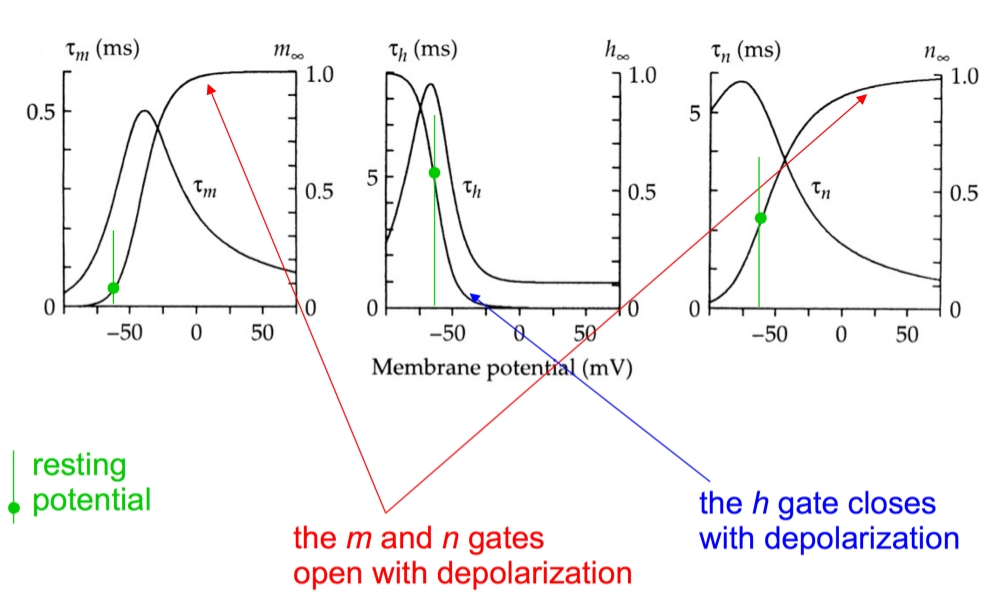
\includegraphics[scale=0.4]{images/5_8.jpg}
  \caption{Gating Variables (from HH Model): voltage - dependence.}
\end{figure} 

\section{Lecture 5 - Action Potential (Valerio Mante)}

% Version Benjamin (Rodney Douglas): reviewed by Dora (Valerio Mante)

\begin{itemize}
\item Voltage Clamp experiment\\
\begin{figure}[htbp]
\centering
  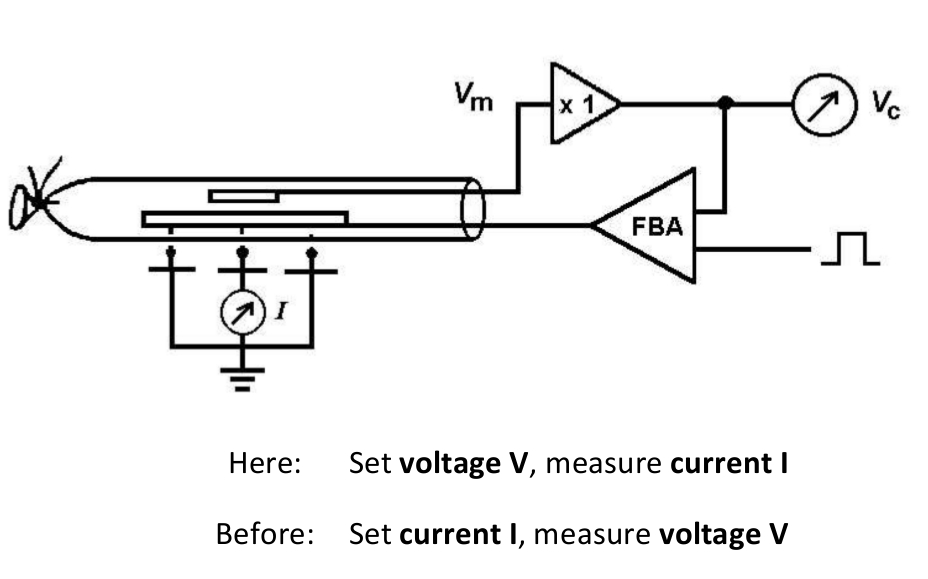
\includegraphics[scale=0.4]{images/5_1.jpg}
\end{figure} 

\item Command voltage is set by the experimenter, the feedback circuit holds the voltage constant.
\item The voltage clamp allows the membrane voltage to be manipulated independently of ionic currents, allowing the current-voltage relationships of membrane channels to be studied.

\begin{figure}[H]
        \centering
        \begin{subfigure}[b]{0.65\textwidth}
                \centering
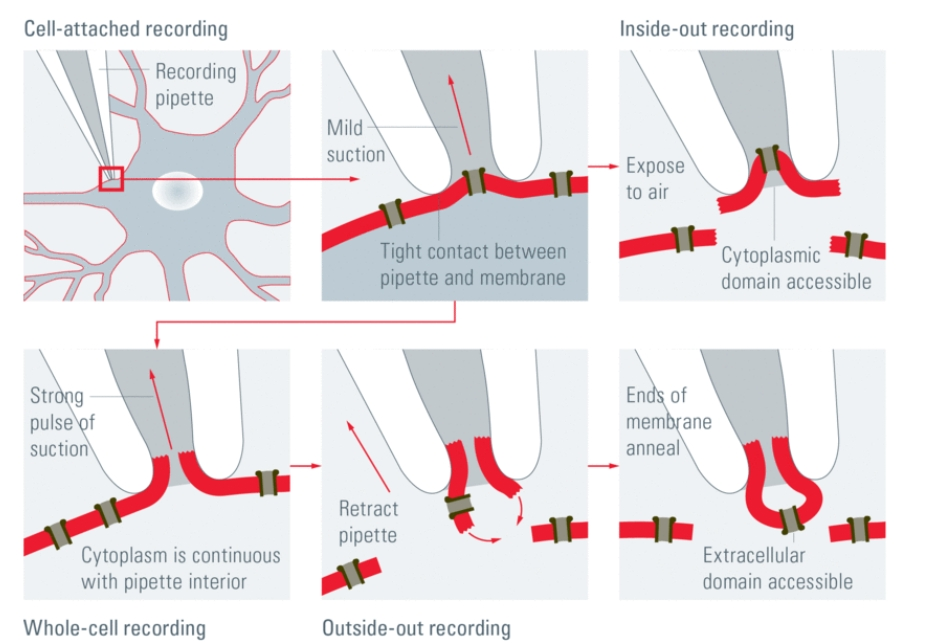
\includegraphics[width=\textwidth]{images/5_2.jpg}
        \end{subfigure}%
        ~
        \begin{subfigure}[b]{0.35\textwidth}
                \centering
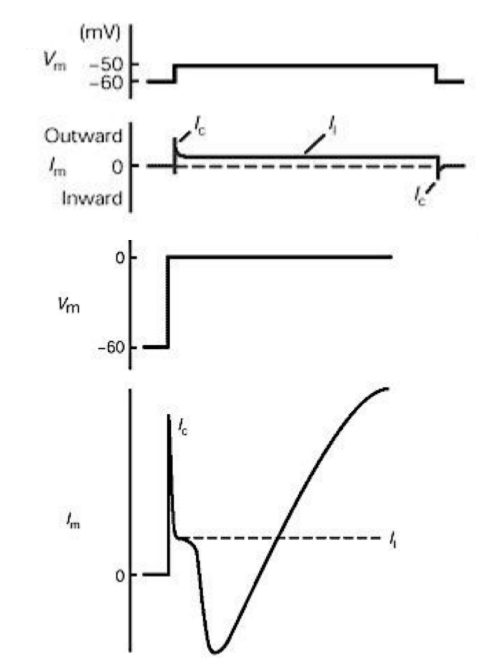
\includegraphics[width=\textwidth]{images/5_3.jpg}
        \end{subfigure}
        \caption{Patch Clamp}
\end{figure}


\item With negative feedback circuit --
The $Na^+$ current is autocatalytic. An increase
in V increases g, which increases the $Na^+$
current, which increases V, etc.

\begin{figure}[htbp]
\centering
  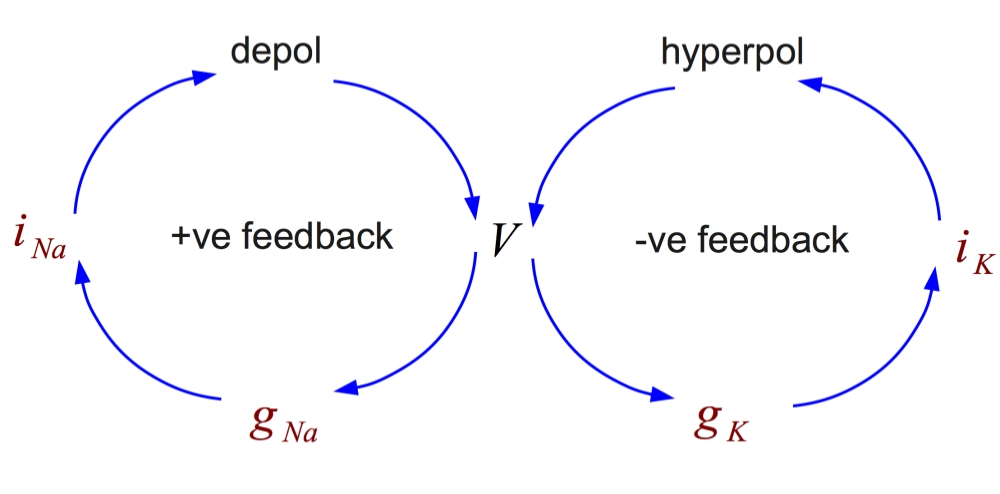
\includegraphics[scale=0.3]{images/5_7.jpg}
  \caption{Feedback mechanism underlie the AP}
\end{figure} 


\item Voltage and time dependent conductances for $g_{Na}, g_{K}$:
\subitem $g_{Na}$ increases quickly, but then inactivation kicks in and it decreases again.
\subitem $g_K$ increases more slowly, and only decreases once the voltage has decreased.
\begin{figure}[H]
        \centering
        \begin{subfigure}[b]{0.65\textwidth}
                \centering
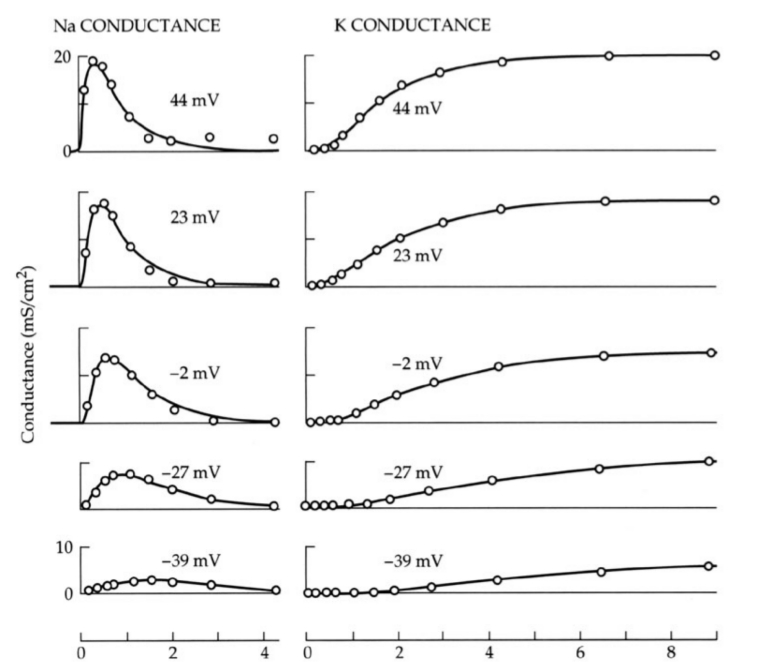
\includegraphics[width=\textwidth]{images/5_4.jpg}
        \end{subfigure}%
        ~
        \begin{subfigure}[b]{0.35\textwidth}
                \centering
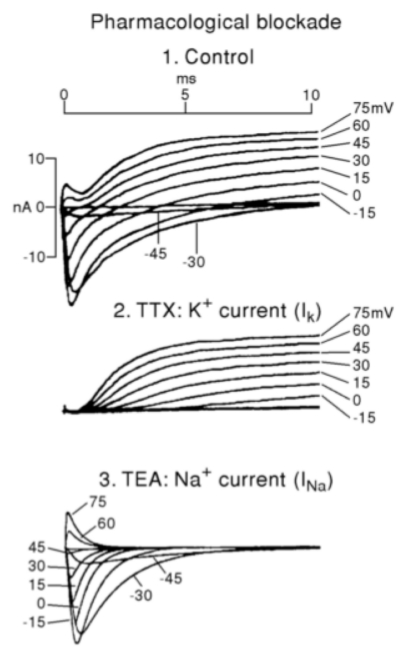
\includegraphics[width=\textwidth]{images/5_4_2.jpg}
        \end{subfigure}
        \caption{From current to conductance}
\end{figure}


\item The threshold for action potential
initiation is where the inward $Na^+$ current
exactly balances the outward $K^+$ current.\\
$\rightarrow g_{Na} > g_K $(leads to the spike[depolarisation]) $\rightarrow g_{K}$ increases $ b                                                                         \rightarrow g_{K} > g_{Na} $(hyperpolarisation)

\item Single Channel current

\begin{figure}[htbp]
\centering
  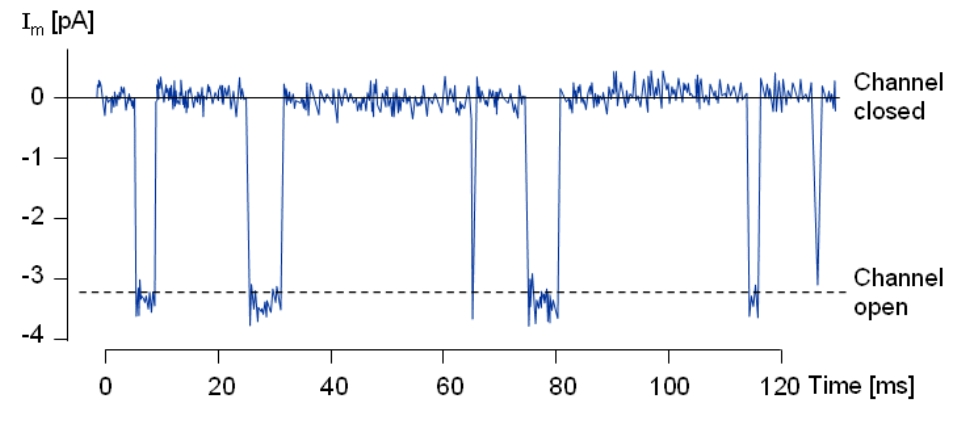
\includegraphics[scale=0.45]{images/5_6.jpg}
\end{figure} 

\item The circuit for action potential generation

\begin{figure}[htbp]
\centering
  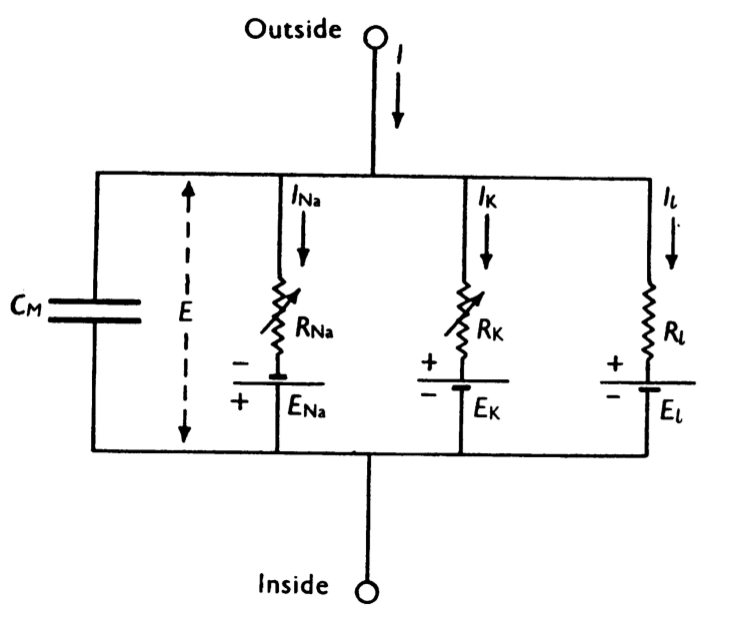
\includegraphics[scale=0.4]{images/5_5.jpg}
\end{figure} 

\end{itemize}


%\begin{figure}[H]
%        \centering
%        \begin{subfigure}[b]{0.6\textwidth}
%                \centering
%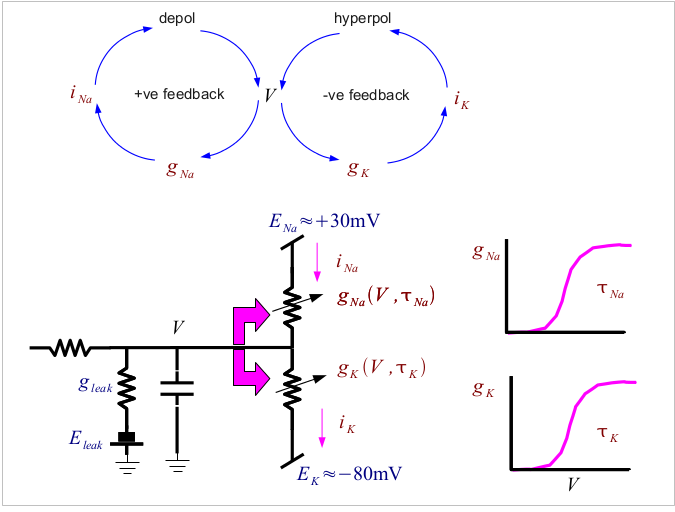
\includegraphics[width=\textwidth]{pos-neg-feedback-loops.png}
%        \end{subfigure}%
%        ~
%        \begin{subfigure}[b]{0.4\textwidth}
%                \centering
%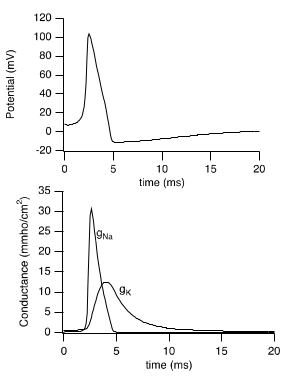
\includegraphics[width=\textwidth]{action-potential.png}
%        \end{subfigure}
%        \caption{The Action potential}
%\end{figure}




%\subsection{The Hodgkin-Huxley equations}
%$C\frac{dV}{dt} + \bar{g}_{K}n^4 (V-V_K)+\bar{g}_{Na}m^3 h(V-V_{Na})+\bar{g}_L(V-V_L) + I_{injected} = 0$\\
%\textbf{$m^3,n^4$} are part of the proposed model.\\
%$\bar{g}_L(V-V_L)$ is the general leak.
%\begin{itemize}
%\item Both amplitude of conductance change and its time const g change with $V_{clamp}$
%\item The m and n gates open with depolarisation
%\item The h gate closes with depolarization\\
%$\rightarrow$ Not symmetrical power (circuit currents),ap goes into one direction
%\end{itemize}

%\subsection{Saltatory conductance}
%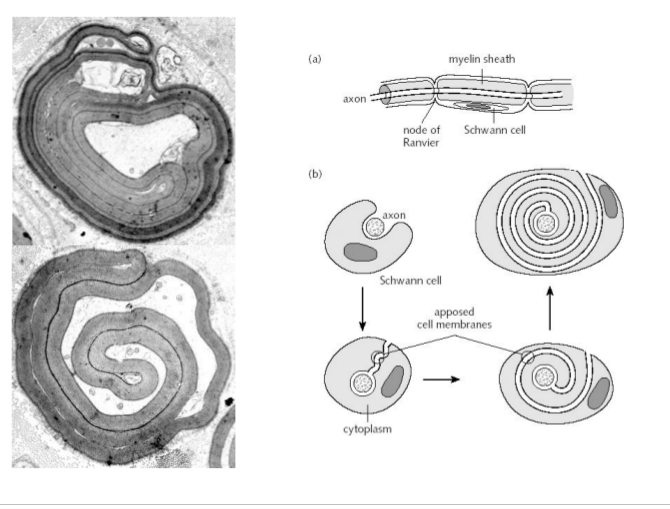
\includegraphics[width=0.7\textwidth]{myelinized-axons.png}
%\begin{itemize}
%\item Ranviernodes 
%\item Myelinized by gliacells $\rightarrow$ resistance high/not leaking
%\item The thicker the cell the faster the signal
%\end{itemize}








\section{Lecture 6 - Synapse 1 (Kevan Martin)}

% Version Benjamin reviewed by Dora:
\begin{itemize}
\item Sherrington (1873)
\subitem First research on synapses. Word "synapse" \& "neuron".
\item Otto Loewi \& Vagus nerve
\subitem Stimulating the vagus nerve slows down the heart beat $\rightarrow$ inhibitory function. (Injection of the solution from 1st heart to 2nd heart).

\begin{center}
Electrical signal $\rightarrow$ chemical signal.
\end{center}

\item Synapse
\subitem Only vesicles which are already on the presynaptic membrane will be released after the AP (not all vesicles are released after an AP)
\subitem One single synapse produces only a small potential. it needs many synapses to create an actual AP. $\rightarrow$ Release of neurotransmitters is Ca dependent.
\item Probabilistic release of neurotransmitter
\subitem in CNS most of the time only one vesicle is released with probability 0.2-0.4
\subitem Amplitude hystogram $\rightarrow$ Poisson distibution $\rightarrow$ probability of firing
(all synapses have probabilistic release).
\subitem Action potential (probability of firing of synapses, probability of postsynaptic receptors to bind neurotransmitter) = \textit{Plasticity} (the overall probability of passing action potential to postsynaptic neurite changes).
\end{itemize}








\section{Lecture 7 - Synapse 2 (Valerio Mante)}

% Version Benjamin reviewed by Dora:
\subsection{Synaptic mechanism}
\begin{enumerate}
\item Synthesis: Building blocks of transmitter substance are imported into the terminal where the neurotransmitter is synthesized and packaged into vesicles.
\item Release: In response to an AP, the transmitter is released across the membrane by exocytosis.
\item Receptor activation: The transmitter crosses the synaptic cleft and binds to a receptor.
\item Inactivation: The transmitter is either taken back into the terminal or inactivated in the synaptic cleft.
\end{enumerate}

\subsection{Categorizing synapses according to:}

\subsubsection{way of activation -- complexity}
\begin{figure}[htbp]
\centering
  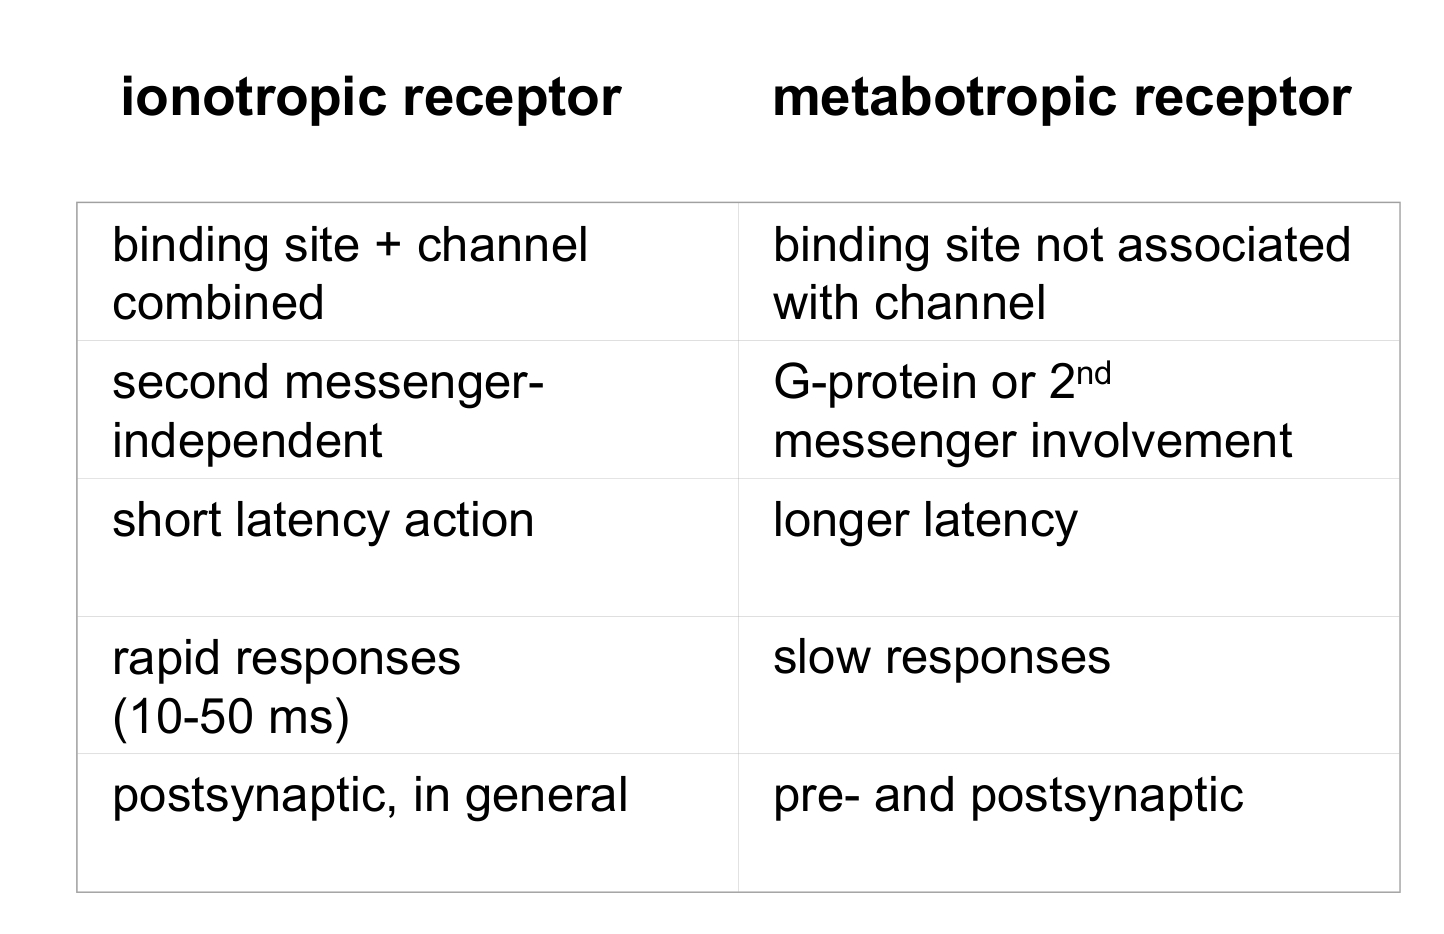
\includegraphics[scale=0.25]{images/6_2.jpg}
\end{figure} 

Ionotropic receptors take part in neurotransmission that involves exclusively ligand-gated ion channels which is much faster (without 2nd messenger).\\
Ligand --  ion or molecule that binds to a central metal atom.

\newpage
\subsubsection{carrier used to transmit information}
\begin{figure}[htbp]
\centering
  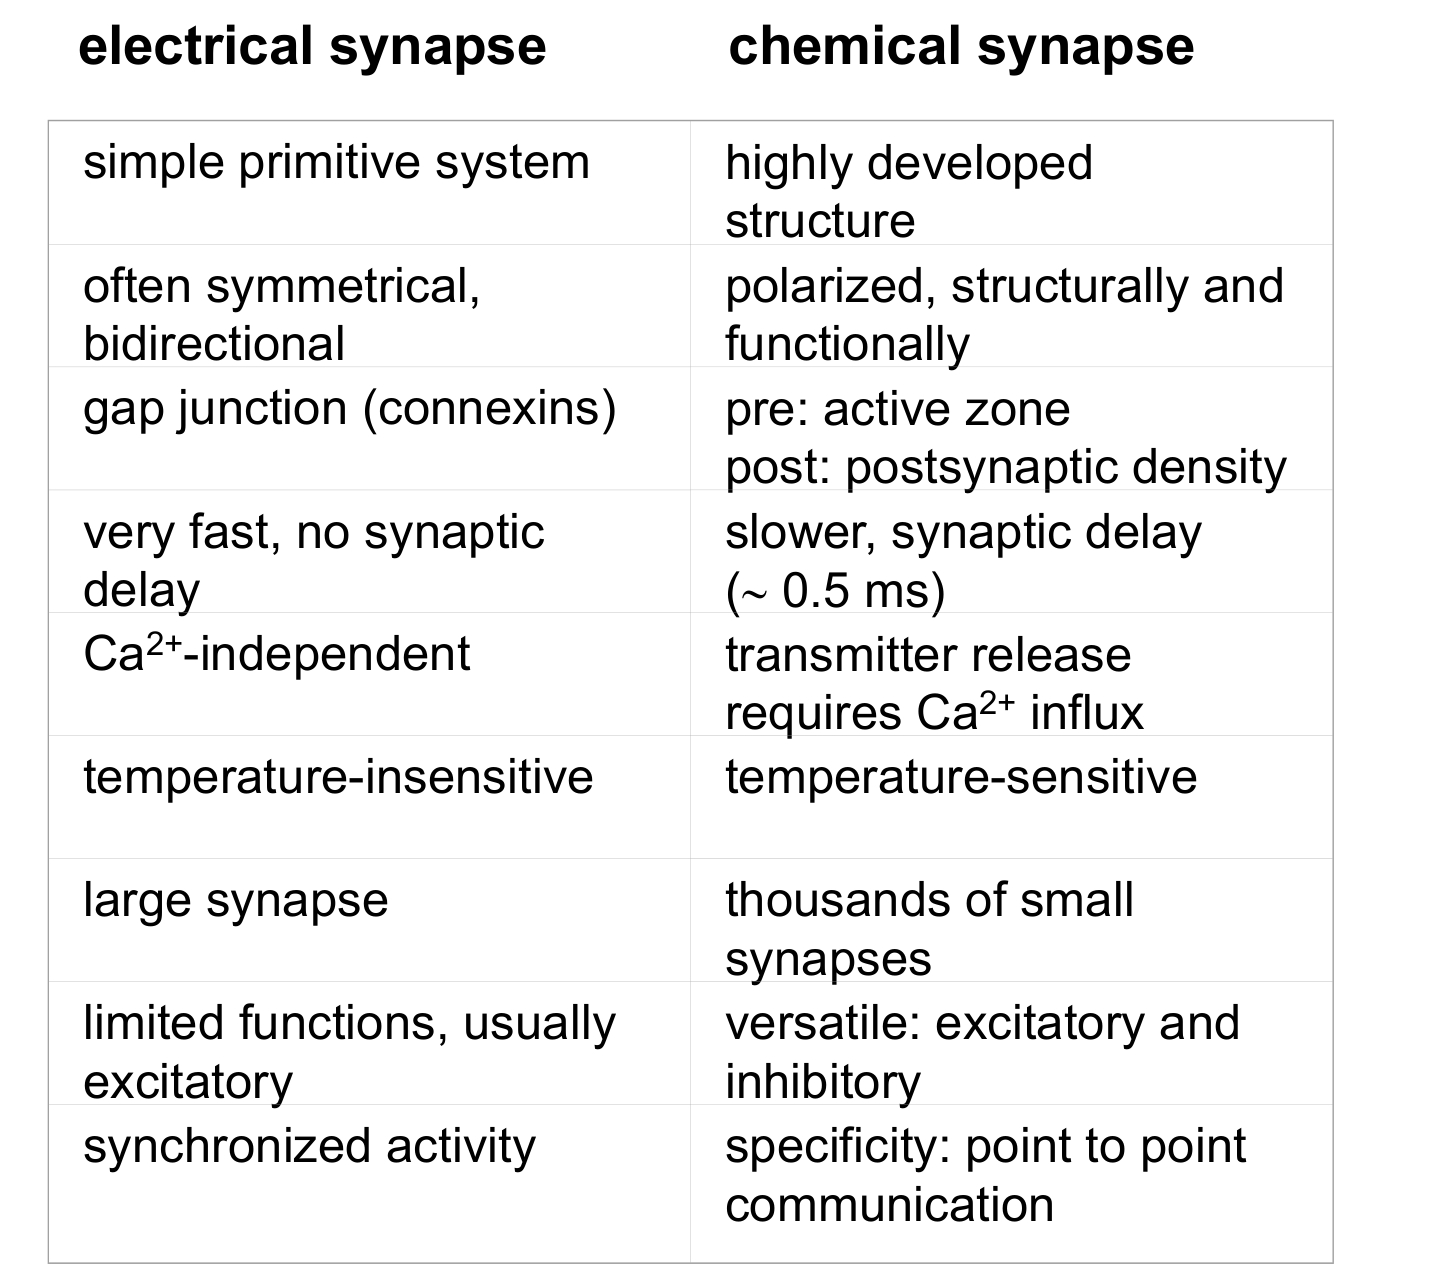
\includegraphics[scale=0.25]{images/6_1.jpg}
\end{figure} 


\subsubsection{function}
\begin{center}
\begin{tabular}{|l|l|}
\hline
Excitatory & Inhibitory\\
\hline
$E_S > E_{Th}$ & $E_S < E_{Th}$ \\
\hline
Glutamate & GABA\\
Ach nic. & ACh musc.\\
\hline
\end{tabular}
\end{center}

Neurotransmitters:
\begin{itemize}
\item ACh
\subitem nicotinic --- $E_s \approx 0mV$, reason why nicotin is addictive $\rightarrow$ fake excitation
\subitem musculinic --- metabotropic -- requires 2nd messanger
\item Glutamine
\subitem AMPA (AMPA receptors bind Glu \& AMPA neurotr.) --- contain $Mg^{2+}$ blocking througput $\rightarrow$  relised by exceeding $30mV$ potential, very fast, $E_s \approx 0mV$
\subitem NMDA (NMDA receptors bind Glu \& NMDA neurotr.) --- ionic transport of $Na^+, K^+$; $Ca^{2+}$ = 2nd messanger; $E_s \approx 0mV$
\item GABA
\subitem $GABA_A$ --- $Cl^-$, ionotropic (fast), $E_s =\approx -65mV$ 
\subitem $GABA_B$ --- $K^+$, metabotropic (slow), $E_s =\approx -90mV$ 
\end{itemize}

\begin{figure}[h]
\begin{center}$
\begin{array}{cc}
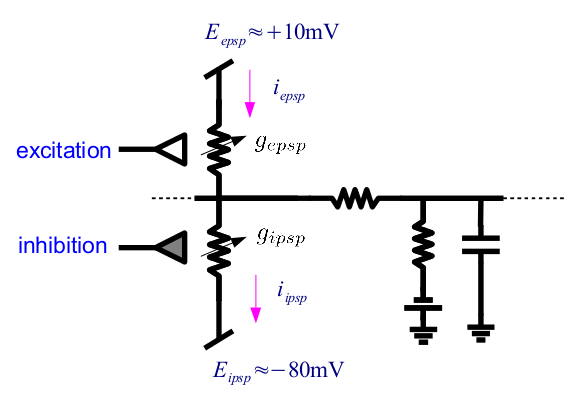
\includegraphics[width=0.5\textwidth]{ex-inhib-elec-membrane.png}
&
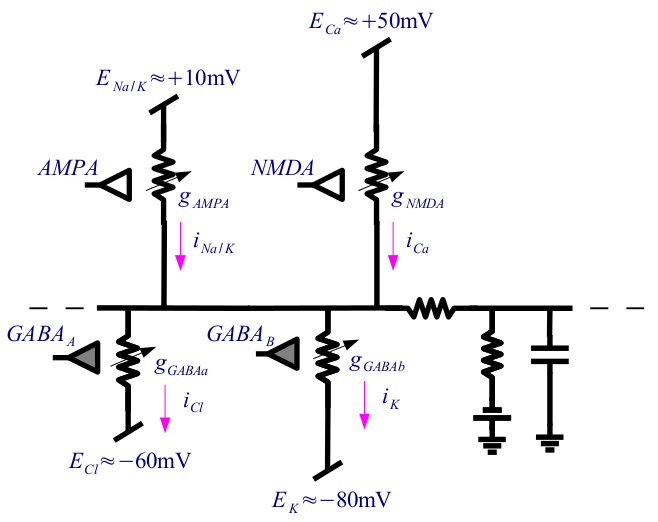
\includegraphics[width=0.5\textwidth]{AMPA-NMDA-GABA-elec-membrane.png}

\end{array}$
\end{center}
\end{figure}

\begin{tabular}{|l|l|l|l|l|l|}
\hline
Receptor & Transmitter & ion & Approx $E_{rev}$ & Agonist\\
\hline
AMPA & glutamate & Na, K, Ca & +0mV & AMPA \\
\hline
	NMDA & glutamate & Ca, Na, K & +0mV & NMDA(glycine) \\
\hline
	mGLU & glutamate & G-coupled & & \\
\hline
	 $GABA_A$ & gaba & Cl & -65mV & muscimol \\
\hline
	 $GABA_B$ & gaba & K & -90mV &  \\
\hline
\end{tabular}

\subsection{Glutamate receptors}


\begin{itemize}
\item AMPA-receptor: Calcium activates NMDA-receptor. Second messenger activates. Weak stimulation by Glutamate only AMPA receptor is bound to Glutamate.\\
$\searrow Na^+,K^+,Ca^{2+}$
\item NMDA-receptor: Depolarization$\rightarrow MG^{2+}$ is removed. Activation by Glutamate and co-agonist $\to Ca^{2+}$ can float in\\
$\searrow Ca^{2+},Na^+,K^+$
\item Important feature of NMDA-receptor
\subitem Activation of glutamate requires co-agonists glycine or serine.
\subitem Effect requires coincidence of depolarization of post-synaptic membrane to dislodge $Mg^{2+}$ and binding of agonist.
\subitem Relatively slow post-synaptic EPSP.
\subitem 10x more permeable to $Ca^{2+}$ than to $Na^+$ or $K^+$
\end{itemize}
\begin{figure}[htbp]
\centering
  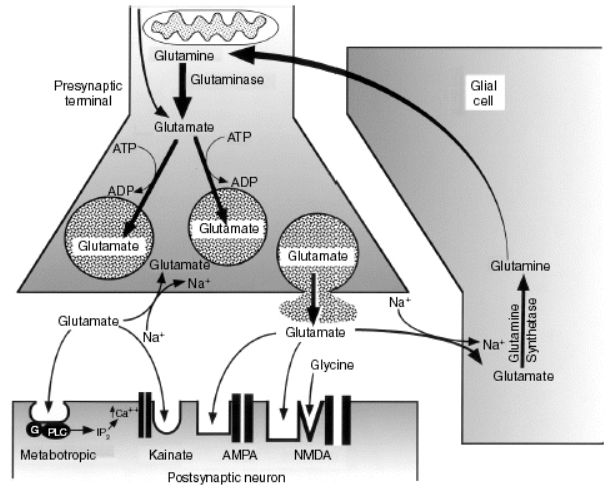
\includegraphics[scale=0.4]{glutamate-neuron.png}
\end{figure} 

\subsection{Neuromodulators **}
Neurotransmitter that is not reabsorbed by the pre-synaptic neuron or broken down into a metabolite. Such neuromodulators end up spending a significant amount of time in the cerebrospinal fluid (CSF), influencing (or "modulating") the activity of several other neurons in the brain, as some neurotransmitters also do (serotonin and acetylcholine).
\begin{itemize}
\item Norepinephrine
\item Dopamine
\item Serotonine
\end{itemize}








\section{Lecture 8 - Plasticity/Learning (Michael Pfeiffer)}

% Version Benjamin reviewed by Dora:

\subsection{Learning \& Memory}
\begin{itemize}
\item Learning is the acquisition of new information or knowledge
\item Memory is the retention of learned information
\item Types of memory
\subitem Declarative Memory (Facts,Events)
\subitem Non-Declarative Memory
\subitem Procedural Memory (Skills, Habits)
\subitem Emotional responses
\item Facts about Synapses
\subitem Neurons communicate via AP and are interconnected via synapses
\subitem Information is represented by distributed activity
\subitem Learning and memory is based on changes in synaptic connections(Formation \& retraction of synapses(development),Changes in synaptics efficacies(plasticity))    
\end{itemize}

\subsection{Plasticity}
What is plasticity?\\
Axiomatic rule: Everything is somehow encoded in synapses.\\
No information in the shape of the spike, but in the frequency and synchronicity.\\
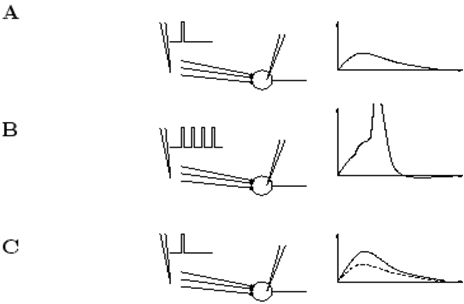
\includegraphics[width=0.8\textwidth]{plasticity.png}
\begin{itemize}
\item Modification of postsynaptic potentials (PSP) evoked by presynaptic spikes
\subitem A. Postsynaptic response triggered by a weak test pulse (left).
\subitem B. Strong stimulation sequence (left) triggers postsynaptic firing.
\subitem C. A later test pulse evokes a larger postsynaptic response than initially.
\item Parameters that define synapse strenghts
\subitem Neurotransmitter and receptor type
\subitem Position of synapse
\subitem Availability of vesicles
\subitem Re-uptake
\subitem Neuromodulators(Dopamin etc.)
\subitem „Non-synaptic“ plasticity(excitablity of neurons, dendritic branch strength)
\subitem Postsynaptic cellular processes
\subitem Pre-/postsynaptic firing
\subitem etc.
\item it is unlikely that there is only one single model that explains all plasticity effects found in biolgy.
\item Diseases affect plasticity: Alzheimer, Parkinson
\end{itemize}


\subsection{Models of plasticity}
\begin{itemize}
\item Non-synaptic plasticity(Excitability of neurons, dendritic branch strength)
\item Synaptic plasticity
\subitem 1.Phenomenological models(High-level,relationships between activity \& plasticity etc. exp: Pavlov Classical conditioning)
\subitem 2.Biophysical models (Low-level,cellular processes etc. exp: Hebbian learning)
\end{itemize}
\subsection{Pavlovian Learning}

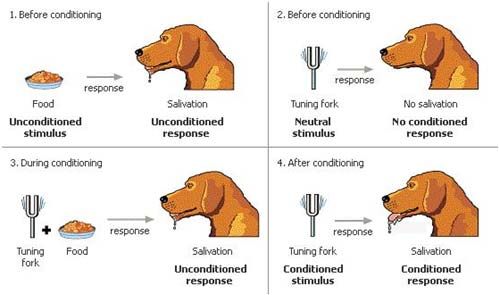
\includegraphics[width=0.8\textwidth]{pavlovian-conditioning.png}

\subsection{Hebbian Learning}
\begin{itemize}
\item "Fire together, wire together"
\item Learning based on correlations between pre- and postsynaptic firing
\item Uses only variables locally available at the synapse
\item Rate-based model: $\Delta synaptic-efficacy_{neuron A,neuron B} \propto firing-rate_{neuron A} \cdot firing-rate_{neuron B}$
\item Only weight increase modelled/No depression\\
$\rightarrow$ Can lead to instability (positive feedback loops)
\item Other rules: BCM rule, Oja's rule
\item Implications:
\subitem Global effects arise from local learning
\subitem Variables(pre- \& postsynaptic action potential,efficacy(weight),local concentration)
\end{itemize}

\subsection{NMDA synapse}
\begin{itemize}
\item Can act as coincidence detector for pre- and postsynaptic firing
\item Backpropagation action potentials
\item Depolarization from other synapses
\item Calcium influx crucial for plasticity
\item Strong NMDA activation $\rightarrow$ potentiation
\item Weak NMDA activation $\rightarrow$ depression
\end{itemize}

\subsection{Short term plasticity(STP)}
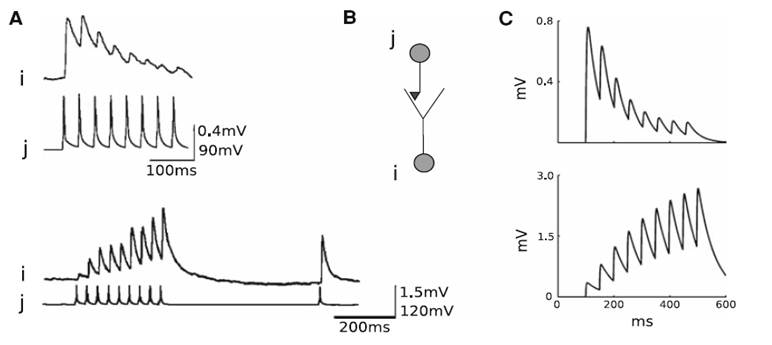
\includegraphics[width=0.8\textwidth]{STP.png}
\begin{itemize}
\item A neuron j fires several times, neuron i fires as well and the spike size is increased(the higher the spike, the more efficient the neuron), but decreases after a short time.(Caused by loss of vesicles)
\item Effect goes away in order of seconds.
\end{itemize}

\subsection{Long term plasticity(LTP)}
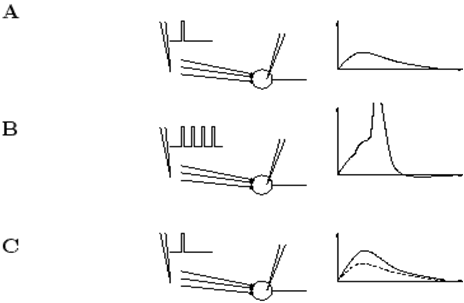
\includegraphics[width=0.8\textwidth]{LTP.png}
\begin{itemize}
\item Schematic drawing of a paradigm of LTP induction. \subitem A. A weak test pulse (left) evokes the postsynaptic response sketched on the right-hand side of the figure. 
\subitem B. A strong stimulation sequence (left) triggers postsynaptic firing (right, the peak of the action potential is out of bounds). 
\subitem C. A test pulse applied some time later evokes a larger postsynaptic response (right; solid line) than the initial response. The dashed line is a copy of the initial response in A. (schematic figure).
\item LTP occurs if a synapse and the post-synaptic neuron are simultaneously depolarized beyond a threshold. This can occur in cooperation (weak and weak or weak and strong signals)
\item 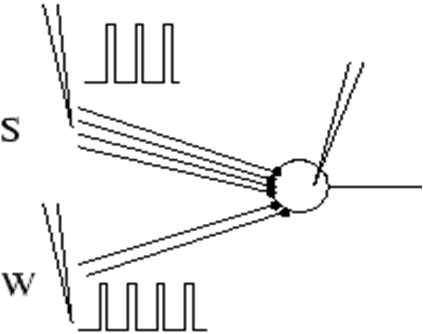
\includegraphics[width=0.5\textwidth]{LTP-coop.png}\\
Cooperativity in the induction of LTP. Weaker synapse W is strengthend if the postsynaptic neuron is active and both presynaptic sites are firing.
\item LTP has a transient early phase (lasting 1-3h) and later phase (24h) demanding new protein and RNA synthesis resulting in the construction of new presynaptic zones and postsynaptic receptors.
\end{itemize}

\subsection{Spike-timing dependent plasticity (STDP)}
\begin{itemize}
\item Not only correlation, but also timing of the spikes determines plasticity.
\item Sign of plasticity is determined by local calcium
concentration
\item Postsynaptic spike travels back to the dendritic tree and activates voltage-dependent Ca channels
\item Presynaptic activity can allow Ca influx through
NMDA channels (if postsynaptic part is sufficiently
depolarized)
\item If pre-spike is soon afterwards followed by post-
spike, NMDA-R activity is supralinearly enhanced by
depolarization due to backpropagating spike
$\rightarrow Ca^{2+}$ determines the strength of plasticity
\item Functional consequence:
\subitem Correlated firing groups win the battle against uncorrelated groups (depression). Battle of two correlated groups have a random winner.\\
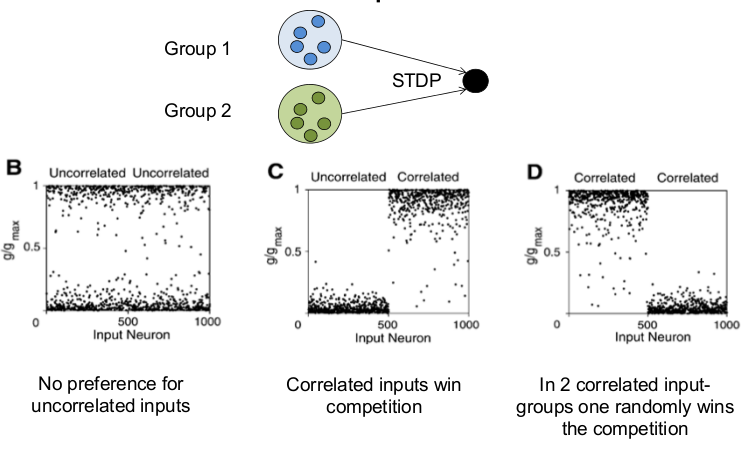
\includegraphics[width=0.8\textwidth]{STDP-consequences.png}
\end{itemize}


\begin{figure}[htbp]
\centering
  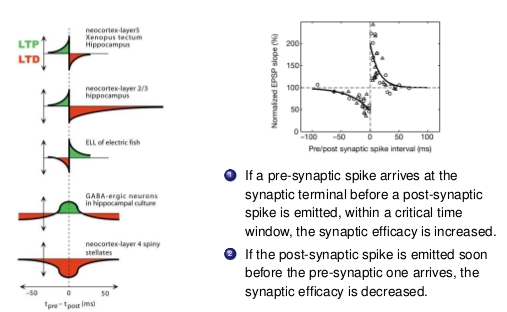
\includegraphics[scale=0.7]{images/8_1.jpg}
\end{figure} 

\subsection{Facts}
\begin{itemize}
\item Different plasticity in different brain areas, diversity in STDP occurances
\item Diversity of neuron and synapse types
\item Large number of control parameters for plasticity experiments (frequency, timing, postsynaptic voltage, position on the dendrite, ...)
\item Influence of neuromodulators, calcium, drugs, and various proteins
\item Long-term vs. short-term effects
\item It is unlikely that there is one single model that explains all plasticity effects found in biology
\end{itemize}

\subsection{Dopamine}
\begin{itemize}
\item Neurotransmitter and neuromodulator, Reinforcement learning
\item Significant for motor processes (Parkinson),pleasure and reward, motivation, attention, emotions
\item DA activation is a relatively
homogeneous, global population signal
\item DA activation is related to rewarding stimuli or reward prediction errors
\item DA can extend
the timing window for LTP, can convert LTD into LTP
\end{itemize}









\section{Lecture 9 - Rate / Event Coding (Michael Pfeiffer)}

%Version Benjamin reviewed by Joachim:

\textbf{What is neural coding?}
\begin{itemize}
\item How is information encoded?
\item Single neuron firing $\leftrightarrow$  Population firing
\item How does a neuron encode information?
\item Firing rate, Timing of spikes
\item What do different measurement techniques tell us about the neural code?
\item Spatial/temporal resolution
\item What is a useful visualization of firings for interpretation?
\end{itemize}
\begin{figure}[H]
        \centering
        \begin{subfigure}[b]{0.5\textwidth}
                \centering
				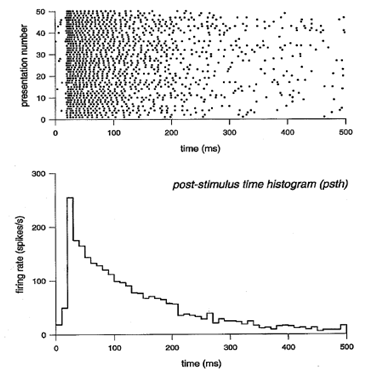
\includegraphics[width=\textwidth]{neural-coding-problem.png}
				\caption{Raster plot = spikes \& Histogram}
        \end{subfigure}%
        ~
        \begin{subfigure}[b]{0.5\textwidth}
                \centering
				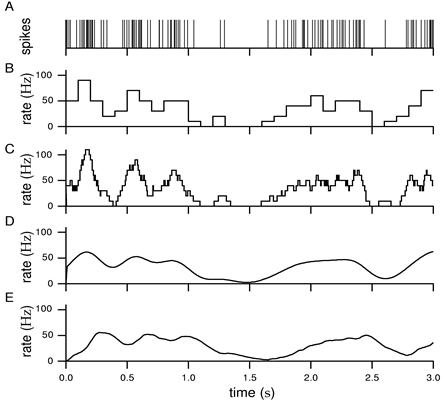
\includegraphics[width=\textwidth]{firing-rate.png}
				\caption{100ms time bins $\rightarrow$ 100ms sliding window $\rightarrow$ gauss filter $\rightarrow$ causal filter}
        \end{subfigure}
\end{figure}


\subsection{Neuronal rate codes(average over time(single neuron))}

\subsubsection*{Tuning curves}
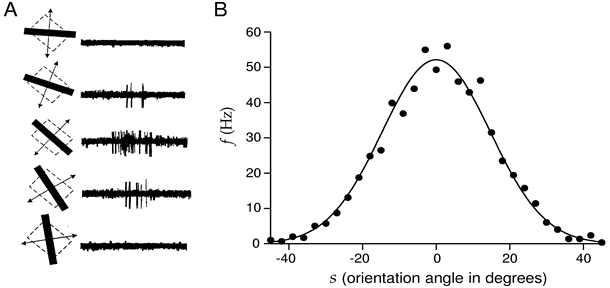
\includegraphics[width=0.9\textwidth]{tuning-curve.png}\\
\begin{itemize}[label={}]\item Shown line and its response primary visual cortex. Turning curve shows average firing rate of varying stimulus parameters. Tuning curves characterize a single cell.\\
\item 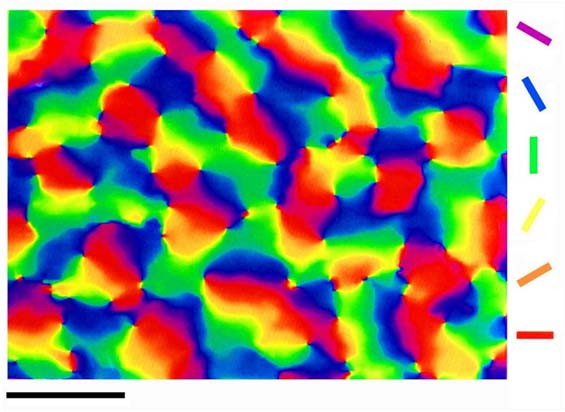
\includegraphics[width=0.7\textwidth]{orientation-map.png}\\
Nearby neurons have similar preferred orientations(colors)\end{itemize}

\subsubsection*{Rate codes}
\begin{itemize}[label={}]
\item + easy to understand 
\item - No timing effects 
\item - Might be misleading 
\subitem More than one stimulus might be encoded
\end{itemize}

\subsection{Poisson Spike Trains }
Mathematical model to describe and generate spike trains (point process)\\
Poisson distribution for the number of spikes in interval $T$ with firing rate $r$:\\
\begin{equation}
P_T (n) =  \frac{(rT)^n}{n!} exp(-rT)
\end{equation}\\
Homogeneous: constant rate $r$\\ 
Inhomogeneous: variable rate $r$\\
Approximation: probability of a spike occurring in short interval of length $\Delta t$: \\
\begin{equation} r(t)\cdot \Delta t \end{equation}


\subsection{What can a single neuron encode?}
\begin{itemize}
\item Places (on entering a particular region)
\item Grids (regularly arranged triangular grid of locations)
\item Head-direction
\item Single cell responds to one single human face (''Grandmother cell'')
\end{itemize}




\subsection{Population rate}

\subsubsection{Population codes}
Different cells encode different range of the stimulus $\rightarrow$ allows accurate reconstruction of the signal (sparse coding,exp. 3 types of color cones in retina)

\begin{itemize}
\item Population vector code\\
Populations of neurons stand for vector directions, encoded direction is vectorial addition weighted by firing rate.
\end{itemize}

\subsubsection{Neuronal Event codes}

\begin{itemize}
\item Time-to-first spike codes
\subitem Can implement competition among different cells
\subitem Can be rank-order code(sequence matters)

\item  Burst- and Temporal Codes\\
Bushcricket auditory neurons in natural environment preserve very high coding precision in extreme noise\\
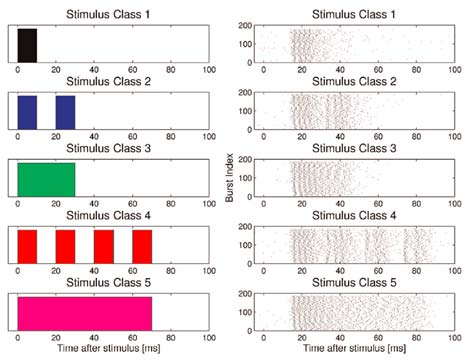
\includegraphics[width=0.7\textwidth]{burst-code.png}

\item  Oscillations and Phase Coding\\
The neurons fire at different phases with respect to the background oscillation\\
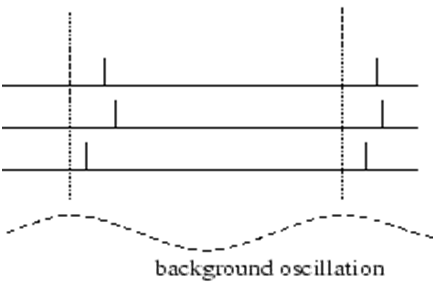
\includegraphics[width=0.6\textwidth]{phase-code.png}

\item  Local Field Potential(LFP)\\
\subitem Low-pass filtered extracellular recording
\subitem Reflects the integration of membrane currents in a local region
\subitem Dominated by dendritic synaptic activity
\subitem Might encode different properties of the stimulus than single cell firing
\subitem Where does it come from / what does it show?
\subitem\includegraphics[width=\textwidth]{MUA-LFP.png}\\
MUA(upper signal) \& LFP (lower signal)
\item  fMRI (functional magnetic resonance imaging)\\ based on blood oxygenation level
\item  Synchrony coding\\
\includegraphics[width=0.6\textwidth]{synchrony-code.png}
\end{itemize}


\subsection{Binding problem}
\includegraphics[width=0.9\textwidth]{binding-problem.png}

\subsection{Averages \& Estimation}

\subsubsection {Spike Triggered Average}
\begin{figure}[H]
        \centering
        \begin{subfigure}[b]{0.5\textwidth}
                \centering
				\includegraphics[width=\textwidth]{spike-triggered-average.png}
				\caption{Average over stimulus in short time window before spike}
        \end{subfigure}%
        ~
        \begin{subfigure}[b]{0.5\textwidth}
                \centering
				\includegraphics[width=\textwidth]{stimulus-estimation.png}
				\caption{Stimulus estimation}
        \end{subfigure}
\end{figure}

\subsubsection {Issues to remember:}
\begin{itemize}
\item Whole stimulus reconstruction may not be relevant
\item Evolution may have shaped us to encode particular features better than others (e.g. faces)
\item Cells may respond to only particular aspects of stimulus
\item Cells may respond to multiple aspects of stimulus
\item Artificial stimuli used for studies may be predictable
\end{itemize}







\section{Lecture 10 - Neuromorphic VLSI(Giacomo Indiveri)} 
%Version Benjamin reviewed by Joachim:
\subsection{VLSI}
\begin{itemize}
\item Very Large Scale Integration Technology allows us to fabricate chips and memory. Digital VLSI( Today's computers) not analog, not low power, not fault tolerant, not robust to inhomogeneities, not asynchronous (clocked), not massively parallel
\item Neuromorphic = VLSI systems containing electronic analog/digital circuits that exploit the physics of silicon to reproduce the bio-physics of neural circuits present in the nervous system. Two main goals:
\subitem To understand the computational properties of biological neural systems using standard CMOS VLSI technology as a tool.
\subitem To exploit the known properties of biological systems to design and implement efficient devices for engineering applications.
\item Neuromorphic VLSI neuron circuits
\subitem To reproduce the physics of neural computation using subthreshold analog circuits and asynchronous digital circuits.
\subitem To build autonomous learning behaving systems that can interact with the environment in real–time
\end{itemize}

\subsection{Why VLSI for neural computation?} 
\begin{itemize}
\item Best exploit current and future VLSI technologies
\item Optimally suited for nano- and future emerging technologies
\item Ideal tools for real- and accelerated-time modeling of neural systems
\item Compact, low-power sensory processing devices for autonomous/flying robots, embedded systems, etc.
\item Direct interface to living systems
\end{itemize}

\subsection{MOSFET Characteristics}
\textbf{n-FET subthreshold transfer function}\\
$I_0$ denotes the nFET current-scaling parameter,\\$\kappa_n$ denotes the nFET subthreshold slope factor,\\$U_T$ the thermal voltage,\\
$V_g$ the gate voltage, $V_s$ the source voltage, and $V_d$ the drain voltage.\\\\
\begin{equation}
I_{ds} = I_0 e^{\frac{\kappa_n V_g}{U_T}}(e^{-\frac{V_s}{U_T}}-e^{-\frac{V_d}{U_T}})
\end{equation}\\
Which is equivalent to\\
\begin{equation}
I_{ds} = I_0 e^{ \frac{\kappa_n V_g}{U_T}-\frac{V_s}{U_T}} - I_0 e^{ \frac{\kappa_n V_g}{U_T}-\frac{V_d}{U_T}}
\end{equation}\\
The first term describes the forward current $I_f$ , the second the reverse current $I_r$\\
\begin{equation}
I_{ds} = I_f - I_r
\end{equation}\\
If $V_{ds} > 4U_T$ the $I_r$ term becomes negligible, and the transistor is said to operate in the saturation regime:\\
\begin{equation}
I_{ds} = I_0 e^{\kappa_n \frac{V_g}{U_T}-\frac{V_s}{U_T}}
\end{equation}\\
\textbf{p-FET subthreshold transfer function}\\
In traditional CMOS circuits, all n-FETs have the common bulk potential ($V_b$) connected to Ground (Gnd), and all p-FETs have a common bulk potential
(typically) connected to the power supply rail ($V_{dd}$ ).
The corresponding (complementary) equation for the p-FET is\\
\begin{equation}
I_{ds} = I_0 e^{\frac{\kappa_p (V_{dd} - V_g)}{U_T}}(e^{-\frac{V_{dd}-V_s}{U_T}}-e^{-\frac{V_{dd}-V_d}{U_T}})
\end{equation}\\
%\frac{g_{d2} g_{dc} }{g_{d2} + g_{sc} } V_0 \approx  \frac{g_{d2} g_{dc} }{g_{d2} + g_{sc} } V_0.


\subsection{Different remarkable circuits}
\begin{itemize}
\item Artificial neuron model by McCulloch \& Pitts
\item Integrate \& fire model (I\&F)
\end{itemize}
\begin{figure}[H]
        \centering
        \begin{subfigure}[b]{0.5\textwidth}
                \centering
\includegraphics[width=\textwidth]{conductance-based-SI-neuron.png}
                \caption{Conductance-based silicon neuron}
        \end{subfigure}%
        ~
        \begin{subfigure}[b]{0.5\textwidth}
                \centering
				\includegraphics[width=\textwidth]{axon-hillock-circuit.png}
                \caption{Axon-Hillock-circuit}
        \end{subfigure}
\end{figure}
\begin{figure}[H]
        \centering
        \begin{subfigure}[b]{0.5\textwidth}
                \centering
\includegraphics[width=\textwidth]{IanF-circuit.png}
                \caption{Ultra low-power generalized I\& F circuit}
        \end{subfigure}%
        ~
        \begin{subfigure}[b]{0.5\textwidth}
                \centering
\includegraphics[width=\textwidth]{multineuron-circuit.png}
                \caption{Spiking multineuron architectures}
        \end{subfigure}
\end{figure}











\section{Lecture 11 - Perceptron Learning Algorithm (Matthew Cook)}


%Version Benjamin reviewed by Joachim:
\includegraphics[width=0.4\textwidth]{perceptron.png}\\
Perceptron, McCulloch-Pitts Neuron, Linear Threshold Unit\\
\begin{itemize}
\item Model represents a neuron as a number of inputs X (dendrites) and one output Y (axon). The weights W determine the influence of a dendrite input, which is either exitatory or inhibitory. f is a function that defines how to combine the weights x and w(normally $\sum (w_i \cdot x_i)$) and $\theta$ (not shown in picture but usually at the place between y and f) is normally a bias that is added to the sum to compare the result to 0.
\item Each neuron has two states: active(1) \& inactive(0)
\item Summing up the products + the bias $\sum x_i\cdot w_i + bias$, then compared to 0 gives us either an ouput of 1 for sums $\ge 0$ or a 0 if < 0.
\item Using this model, we can create conventional electronic gates such as AND-Gate, OR-Gate and NOT-Gate. 
\item However the XOR-Gate/NXOR-Gate is not possible in this model. Both functions are not linear.
\end{itemize}


\subsection{Logic Gates}

\begin{longtable}[t width=1 \textwidth]{ l c r }

  AND & \raisebox{-.5\height}{\includegraphics[]{100px-AND_ANSI.png}} & \raisebox{-.5\height}{\includegraphics[]{table_and.png}} \\
  \noalign{\smallskip}
  OR & \raisebox{-.5\height}{\includegraphics[]{100px-OR_ANSI.png}} & \raisebox{-.5\height}{\includegraphics[]{table_or.png}} \\
  \noalign{\smallskip}
  NOT & \raisebox{-.5\height}{\includegraphics[]{100px-NOT_ANSI.png}} & \raisebox{-.5\height}{\includegraphics[]{table_not.png}} \\
  \noalign{\smallskip}
  XOR & \raisebox{-.5\height}{\includegraphics[]{100px-XOR_ANSI.png}} & \raisebox{-.5\height}{\includegraphics[]{table_xor.png}} \\
  \noalign{\smallskip}
  NAND & \raisebox{-.5\height}{\includegraphics[]{100px-NAND_ANSI.png}} & \raisebox{-.5\height}{\includegraphics[]{table_nand.png}} \\
  \noalign{\smallskip}
  NOR & \raisebox{-.5\height}{\includegraphics[]{100px-NOR_ANSI.png}} & \raisebox{-.5\height}{\includegraphics[]{table_nor.png}} \\
  \noalign{\smallskip}
  XNOR & \raisebox{-.5\height}{\includegraphics[]{100px-XNOR_ANSI.png}} & \raisebox{-.5\height}{\includegraphics[]{table_xnor.png}} \\
\end{longtable}


\subsection{Why XOR is Impossible with Perceptrons}
Consider a perceptron with two inputs, $x_1$ and $x_2$, and an output $y$.\\$x_1$ has weight $w_1$ and $x_2$ has weight $w_2$, and of course we have a threshold $t$\\ \\
\begin{center}
XOR-Table\\
\begin{tabular}[t width=1 \textwidth]{ |l| |c| |r| }
\hline & & \\ $x_1$ & $x_2$ & $y$\\ \hline
0 & 0 & 0\\ \hline
0 & 1 & 1\\ \hline
1 & 0 & 1\\ \hline
1 & 1 & 0\\ \hline
\end{tabular}\\[2\baselineskip]
$0 \cdot w_1 + 0 \cdot w_2 < t \rightarrow y=0$ \\
$0 \cdot w_1 + 1 \cdot w_2 \ge t \rightarrow y=1$ \\
$1 \cdot w_1 + 0 \cdot w_2 \ge t \rightarrow y=1$ \\
$1 \cdot w_1 + 1 \cdot w_2 < t \rightarrow y=0$ \\[2\baselineskip]
This causes a contradiction:\\
$w_1 \ge t$ \\
$w_2 \ge t$ \\
$0 < t$\\
$w_1 + w_2 < t$


\end{center}

\subsection{Comparison Perceptrons vs. Real Neurons}

\begin{itemize}
\item Similarities to biological neurons
\subitem Active or inactive state
\subitem Directionality(input/output)
\subitem Activity dependent of weighted functions of other neurons
\item Differences to biological neurons
\subitem Continous time vs. discrete time
\subitem Degrees of activation
\subitem Activation as a function of the inputs of a real neuron is not linear.
\end{itemize}

\subsection{Perceptron Learning Algorithm}
Given a set of (input vector$x_i$, desired output$d_i$) pairs, finds weights that produce the desired output$d_i$.(If such weights exist)\\
\begin{itemize}
\item Choose random weights
\item Calculate actual output.
\item $y_i = f[w(t)\cdot x_j] = \sum w_i \cdot x_i$ + bias
\item If wrong output $\rightarrow$ change weights
\item For every weight $w_i(t+1) = w_i(t) + \alpha(d_j-y_j(t))x_i$
\item This is repeated until the iteration error $\frac{1}{s}\sum_j^2[d_j-y_j(t)]$ is less than a user-specified error threshold $\gamma$ or until we completed a predefined numer of iteration.
\item Algorithm creates a sufficient result if a solution exists.
\end{itemize}

\subsection*{Example}
(copied from http://en.wikipedia.org/wiki/Perceptron)\\
A perceptron learns to perform a binary NAND function on inputs $x_1$ and $x_2$.\\ $x_0$ held constant at 1\\
Threshold ($t$): 0.5\\Bias ($b$): 0\\Learning rate ($r$): 0.1\\
Training set, consisting of four samples:$\{ ((0,0),1),((0,1),1),((1,0),1),((1,1),0) \}$\\
In the following, the final weights of one iteration become the initial weights of the next. Each cycle over all the samples in the training set is demarcated with heavy lines.\\

\begin{figure}[h!]
  %\caption{Iterations of a perceptron. Copied from http://en.wikipedia.org/wiki/Perceptron}
  \centerline{\includegraphics[width=1.5\textwidth]{perceptron_example.png}}
\end{figure}




\section{Lecture 12 - Hopfield Networks(Matthew Cook)}
%Version Benjamin reviewed by Joachim (some parts copied from Doris Ling):
\subsection*{Key properties of associative memory}
\begin{itemize}
\item Room for error, but still recognizable
\subitem If some units are retreivable \& all others set randomly, the correct units will eventually set wrong units right
\subitem how actual memory works (reliable but boundaries/limits not well defnied)
\item not stored in list
\item Converges to nearby stable states
\subitem Only helpful if reliable input
\end{itemize}

In a Hopfield network (a recurrent network), every node is connected to every other node but not to itself.
The nodes therefore form a single layer. The entire network is in some state at any time. The important readout is therefore the state (set of active units) of the entire network rather than the value of some output nodes in other network types.
Some of the states are stable and some are not. While the network is not in a stable state, updating the network leads to a state change that ultimately converges to a certain stable state (local minimum).\\
\subsection*{Features:}
A hopfield network is an associative type of memory just as the human memory and is able to remember states it learned before. A Hopfield network of 100 nodes can store about approximately 15 pictures(stored as local minima in the network or stable states). Important is that the pictures are distinct, otherwise it can be that the network gets new stable states and the pictures only get ''half remembered''.\\
\includegraphics[width=0.4\textwidth]{hopfield-network-face-recog.png}


\subsection*{Important properties of Hopfield networks}
\begin{itemize}
\item Each node has a value of -1/1 or 0/1. It is therefore active or inactive.
\item Weight of  a conncetion is correlated to frequency of firing together (Hebbian learning)
\item Symmetric, conncetion weight is the same regardless of direction
\subitem \begin{itemize} \item If Node A is connected to Node B via conncetion $C_{AB}$ and Node B is connected to Node A via conncetion $C_{BA}$, then weight of $C_{AB}$ equals weight of $C_{BA}$ \end{itemize}
\item Feedback loops, but no conncetion to itself (cannot feedback on itself)
\item No quantitative description (formula)
\item Nodes can be updated synchronously or asynchronously
\end{itemize}

\subsection{Updates and State Dynamics}
\begin{itemize}[label={}]
\item State: Set of units that are active
\item Dynamics: Units Update their activity level
\end{itemize}
When we update a node,we consider weights to that node from all other active nodes (nodes with value 1).
If the sum of all weights of the active nodes is higher than zero then this neuron is active too.
Updates: can be synchronous (all together) or asynchronous (one at a time)
\begin{itemize}[label={}] \item Asynchrous updates converges to astable state
\item Asynchronous updates are done with a greedy algorithm
\subitem Activities in $\{0,1\}$ $\rightarrow$ Network (approx weighted\\ graph w. weighted edges (maximized)) operation is greedy max-clique)
\subitem Activities in $\{-1,1\}$ $\rightarrow$ Network operation is greedy min-cut
\item Synchronous update converges to a pair of patterns (flipping) or converge to stable state
\item Activities in $\{0,1\}$ $\rightarrow$	Network (approx weighted graph w. \\weighted edges (maximized)), operation is greedy max-clique
\item Activities in $\{-1,1\}$ $\rightarrow$ Network operation is greedy min-cut
\end{itemize}
Update function:\\
$a_{i,t}$ = output of unit at time t\\\\
$a_{i,t+1} =
\left\{
	\begin{array}{ll}
		1   & \sum_{j=1}^N a_{i,t}\cdot w_{ij} > \theta_i (\mbox{often 0}) \\
		-1 & \mbox{otherwise}
	\end{array}
\right.$



\includegraphics[width=0.7\textwidth]{hopfield-network.png}\\
%TODO Example








\section{Lecture 13 - Feed-Forward Networks (Matthew Cook)}

%Version Benjamin reviewed by Joachim (using notes from Doris Ling):

Feed-Forward Network with back-propagation is a network that is single-directed(multiple layers of nodes) and has a certain number of inputs x and a certain number of outputs f. Every layer of nodes ''feeds'' the next layer with information.\\
\includegraphics[width=0.3\textwidth]{Feed_forward_neural_net.png}\\
FFN are helpful if known input $\&$ output pairs exists, we therefore only have to adjust the weights. This procedure is called training or learning.
In many applications the nodes use a sigmoid function as an activation function.\\[2\baselineskip]

\subsection{Error Function}
To evaluate the performance of the newtork we use an error function:\\
\begin{equation}
E(\vec{w})=\sum_{(input,output)_{pairs}}\text{error in output}
\end{equation}
\begin{center}
where $A_1...A_n$ are the values of the output nodes\\$\vec{w}$ = weights of function
\end{center}
\begin{equation}
E(\vec{w})= [(\text{network output})-(\text{desired output})]^2
\end{equation}\\
\begin{equation}
E(\vec{w})= [(A_1,A_2,...,A_n)-(D_1,D_2,...,D_n)]^2
\end{equation}\\
\begin{equation}
E(\vec{w})= (A_1-D_1)^2+(A_1-D_1)^2+...+(A_n-D_n)^2
\end{equation}\\

\subsection{Improve Error}
To improve the error, we need to adjust $\vec{w}$, ie: calculate $\frac{\delta E}{\delta w_i}$ for each i.\\
This is, however, not particulary helpful for reconstruction $f(x)$ because $\frac{\delta f^2}{\delta}=0$ everywhere.\\
We have to use units with continous range of outputs:\\

\begin{figure}[h!]
  
  \centerline{\includegraphics[width=0.5\textwidth]{fnn_hard_threshold.png} \includegraphics[width=0.5\textwidth]{fnn_soft_threshold.png}}
\end{figure}



\begin{equation}
\begin{array}[width=1\textwidth]{lr}
\theta_n(x) = \left\{  \begin{array}{l l} 0 & \quad \text{if } x < 0\\1 &  \quad\text{if } x \ge 0 \end{array}\quad\quad\quad\quad \right.\quad & \quad\theta_s(x) =   \frac{e^x}{1+e^x} 
\end{array}
\end{equation}\\
\begin{center}
\includegraphics[]{fnn_node.png}\\
\begin{equation}
a_4 = \theta_s (a_1w_1 + a_2w_2 + a_3w_3)
\end{equation}\\
\begin{equation}
\text{where: }\begin{array}[width=1\textwidth]{lr}
\frac{\delta a_4}{\delta a_1}= \theta_s'(\vec{A}\cdot\vec{w})\cdot w_1 & \text{ and } \frac{\delta a_4}{\delta w_1}= \theta_s'(\vec{A}\cdot\vec{w})\cdot a_1
\end{array}
\end{equation}\\

\begin{equation}
\frac{\delta a_4}{\delta w_0} = \theta_s'(\vec{A}\cdot\vec{w})\cdot
\end{equation}\\
\end{center}

\textbf{Error of network:}\\
Knowing desired output $D_{p,i}$ can adjust weights in previous activity layer\\
$\rightarrow$ use adjusted activity to adjust weights in previous layer until $A_{i,p}=D_{i,p}$\\
$\Longrightarrow$ Back-Propagation Algorithm\\
$\rightarrow$ useful because we do not need to know network specifics $\rightarrow$ network can learn on its own.\\

\begin{center}
\begin{equation}
\frac{\delta E}{\delta w_1} = \sum_{p,i} 2(A_{i,p}-D{i,p}) \frac{\delta A_{i,p}}{\delta w_1}
\end{equation}\\
\begin{equation}
A_4 \rightarrow \frac{\delta E}{\delta A_4}
\end{equation}\\
\begin{equation}
\frac{\delta E}{\delta w_1} = \sum_{\text{target units i}} \frac{\delta E}{\delta A_i} \cdot \frac{\delta A_{i}}{\delta A_4}
\end{equation}\\
\includegraphics[]{fnn_network.png}\\
\end{center}

\subsection{Back Propagation Algorithm}

Back-propagation is a way method that lets information flow backwards inside of the single directed network. It improves the weight via gradient descent. The back flow of information seems not to be the way biology is doing it. It is a learning technique that compares the output values $f_i$ to the desired values $g_i$ to compute corrective values with a predefined error function.\\\\
$E = \sum (f_i -g_i)^2$\\

The error is then propagated back through the network to adjust the weights of each connection to reduce the deviation from the desired values. The network will converge to either no or just a small error.\\[2\baselineskip]
To adjust weights properly, one optimizes by a method called gradient descent:\\\\
$\frac{\delta E}{\delta w_k} = \sum 2(f_i - g_i) \cdot \frac{\delta(f_i - g_i}{\delta w_k} = \sum 2(f_i - g_i) \frac{\delta f_i}{\delta w_k}$\\[2\baselineskip]
Feed inputs to network one at a time. Compare output to desired output \\\\$f_i - g_i$\\[2\baselineskip]
For each weight, compute the sensitivity of output \\\\$\frac{\delta f_i}{\delta w_k}$\\[2\baselineskip]
Adjust weights \\\\$w_k$ by $\epsilon \cdot (f_i - g_i) \frac{\delta f_i}{\delta w_k}$


%TODO Example




\section{Lecture 14 - Interacting Neural Populations(Matthew Cook)}
%Version Benjamin reviewed by Joachim:
Neurons represent information in many ways, and many of them are unknown. One way os represenation is through population code.

\subsection{Population codes}
Idea: Information is represented by the pattern of activity in a neural population. Specially, neurons are ''tuned'' to preferred stimuli.\\
The population represents a value (or several), e.g. the orientation of a line. Here, each neuron has a preferred orientation that it responds to. We say it is "tuned" to this value. Neurons of similar tuning are grouped together in some species (e.g. in cats), in others they seem to be distributed randomly (e.g. in squirrels).
\begin{itemize}[label={}]
\item We train a monkey to hold its gaze fixed while we move a visual stimulus around. The monkey holds its gaze fixed at E = \colorbox{magenta}{$-15^\circ$}/\colorbox{green}{$0^\circ$}/\colorbox{blue}{$15^\circ$}(eye angle) while we move the stimulus from R =$-40^\circ ... 40^\circ$ (retinal angle).
\end{itemize}

\begin{figure}[H]
        \centering
        \begin{subfigure}[b]{0.3\textwidth}
                \centering
\includegraphics[width=\textwidth]{one-cell-tuning-curve.png}
                \caption{Tuning curve of one cell}
        \end{subfigure}%
        ~
        \begin{subfigure}[b]{0.3\textwidth}
                \centering
\includegraphics[width=\textwidth]{cell-order.png}
                \caption{Cells ordered by response to $20^\circ$}
        \end{subfigure}
        ~ 
        \begin{subfigure}[b]{0.3\textwidth}
                \centering
				\includegraphics[width=\textwidth]{3D-visualisation.png}
                \caption{3D visualization of cell's response to different degrees}
        \end{subfigure}
\end{figure}

\begin{figure}[H]
        \centering
        \begin{subfigure}[b]{0.5\textwidth}
                \centering
\includegraphics[width=\textwidth]{ape-picture.png}
                \caption{Monkey holding gaze fixed on point $10^\circ$ and light falling in from $20^\circ$}
        \end{subfigure}%
        ~
        \begin{subfigure}[b]{0.5\textwidth}
                \centering
				\includegraphics[width=\textwidth]{Retina-Eye-Auditory.png}
                \caption{Visualization of Retina angle ordering cell set R, Eye angle ordering set E,2D result population C and auditory direction set A.}
        \end{subfigure}
\end{figure}

\begin{figure}[H]
        \centering
        \begin{subfigure}[b]{0.3\textwidth}
                \centering
				\includegraphics[width=\textwidth]{Cell-A.png}
                \caption{Cell A $\in$ R}
        \end{subfigure}%
        ~
        \begin{subfigure}[b]{0.3\textwidth}
                \centering
				\includegraphics[width=\textwidth]{Cell-B.png}
                \caption{Cell B $\in$ A}
        \end{subfigure}
        ~ 
        \begin{subfigure}[b]{0.3\textwidth}
                \centering
                \includegraphics[width=\textwidth]{Cell-C.png}
				\caption{Cell C $\in$ E}
        \end{subfigure}
\end{figure}

\begin{figure}[H]
        \centering
        \begin{subfigure}[b]{0.3\textwidth}
                \centering
				\includegraphics[width=\textwidth]{Cell-D.png}
                \caption{Cell D $\in$ C}
        \end{subfigure}%
        ~
        \begin{subfigure}[b]{0.3\textwidth}
                \centering
				\includegraphics[width=\textwidth]{Cell-E.png}
                \caption{Cell E (Not every neuron shows clear tuning curves)}
        \end{subfigure}
\end{figure}






\end{document}
